\appendixpageoff
\begin{appendices}
%Agregar los apéndices

%\chapter*{Anexo A}
%\addcontentsline{loa}{appendix}{Anexo A: Titulo del anexo A}

%Aquí el contenido del anexo A

%\chapter*{Anexo B: El uso de plantillas}
%\addcontentsline{loa}{appendix}{Anexo B: El uso de plantillas}

%Aquí el contenido del anexo B
% \chapter*{Anexo A}
% \addcontentsline{loa}{appendix}{Anexo A: Mapa batimetr\'ico del lago Ypakarai}
% \label{appendix: mapas}

% \setcounter{figure}{0}    

% \begin{figure}[ht]
%     \centering
%     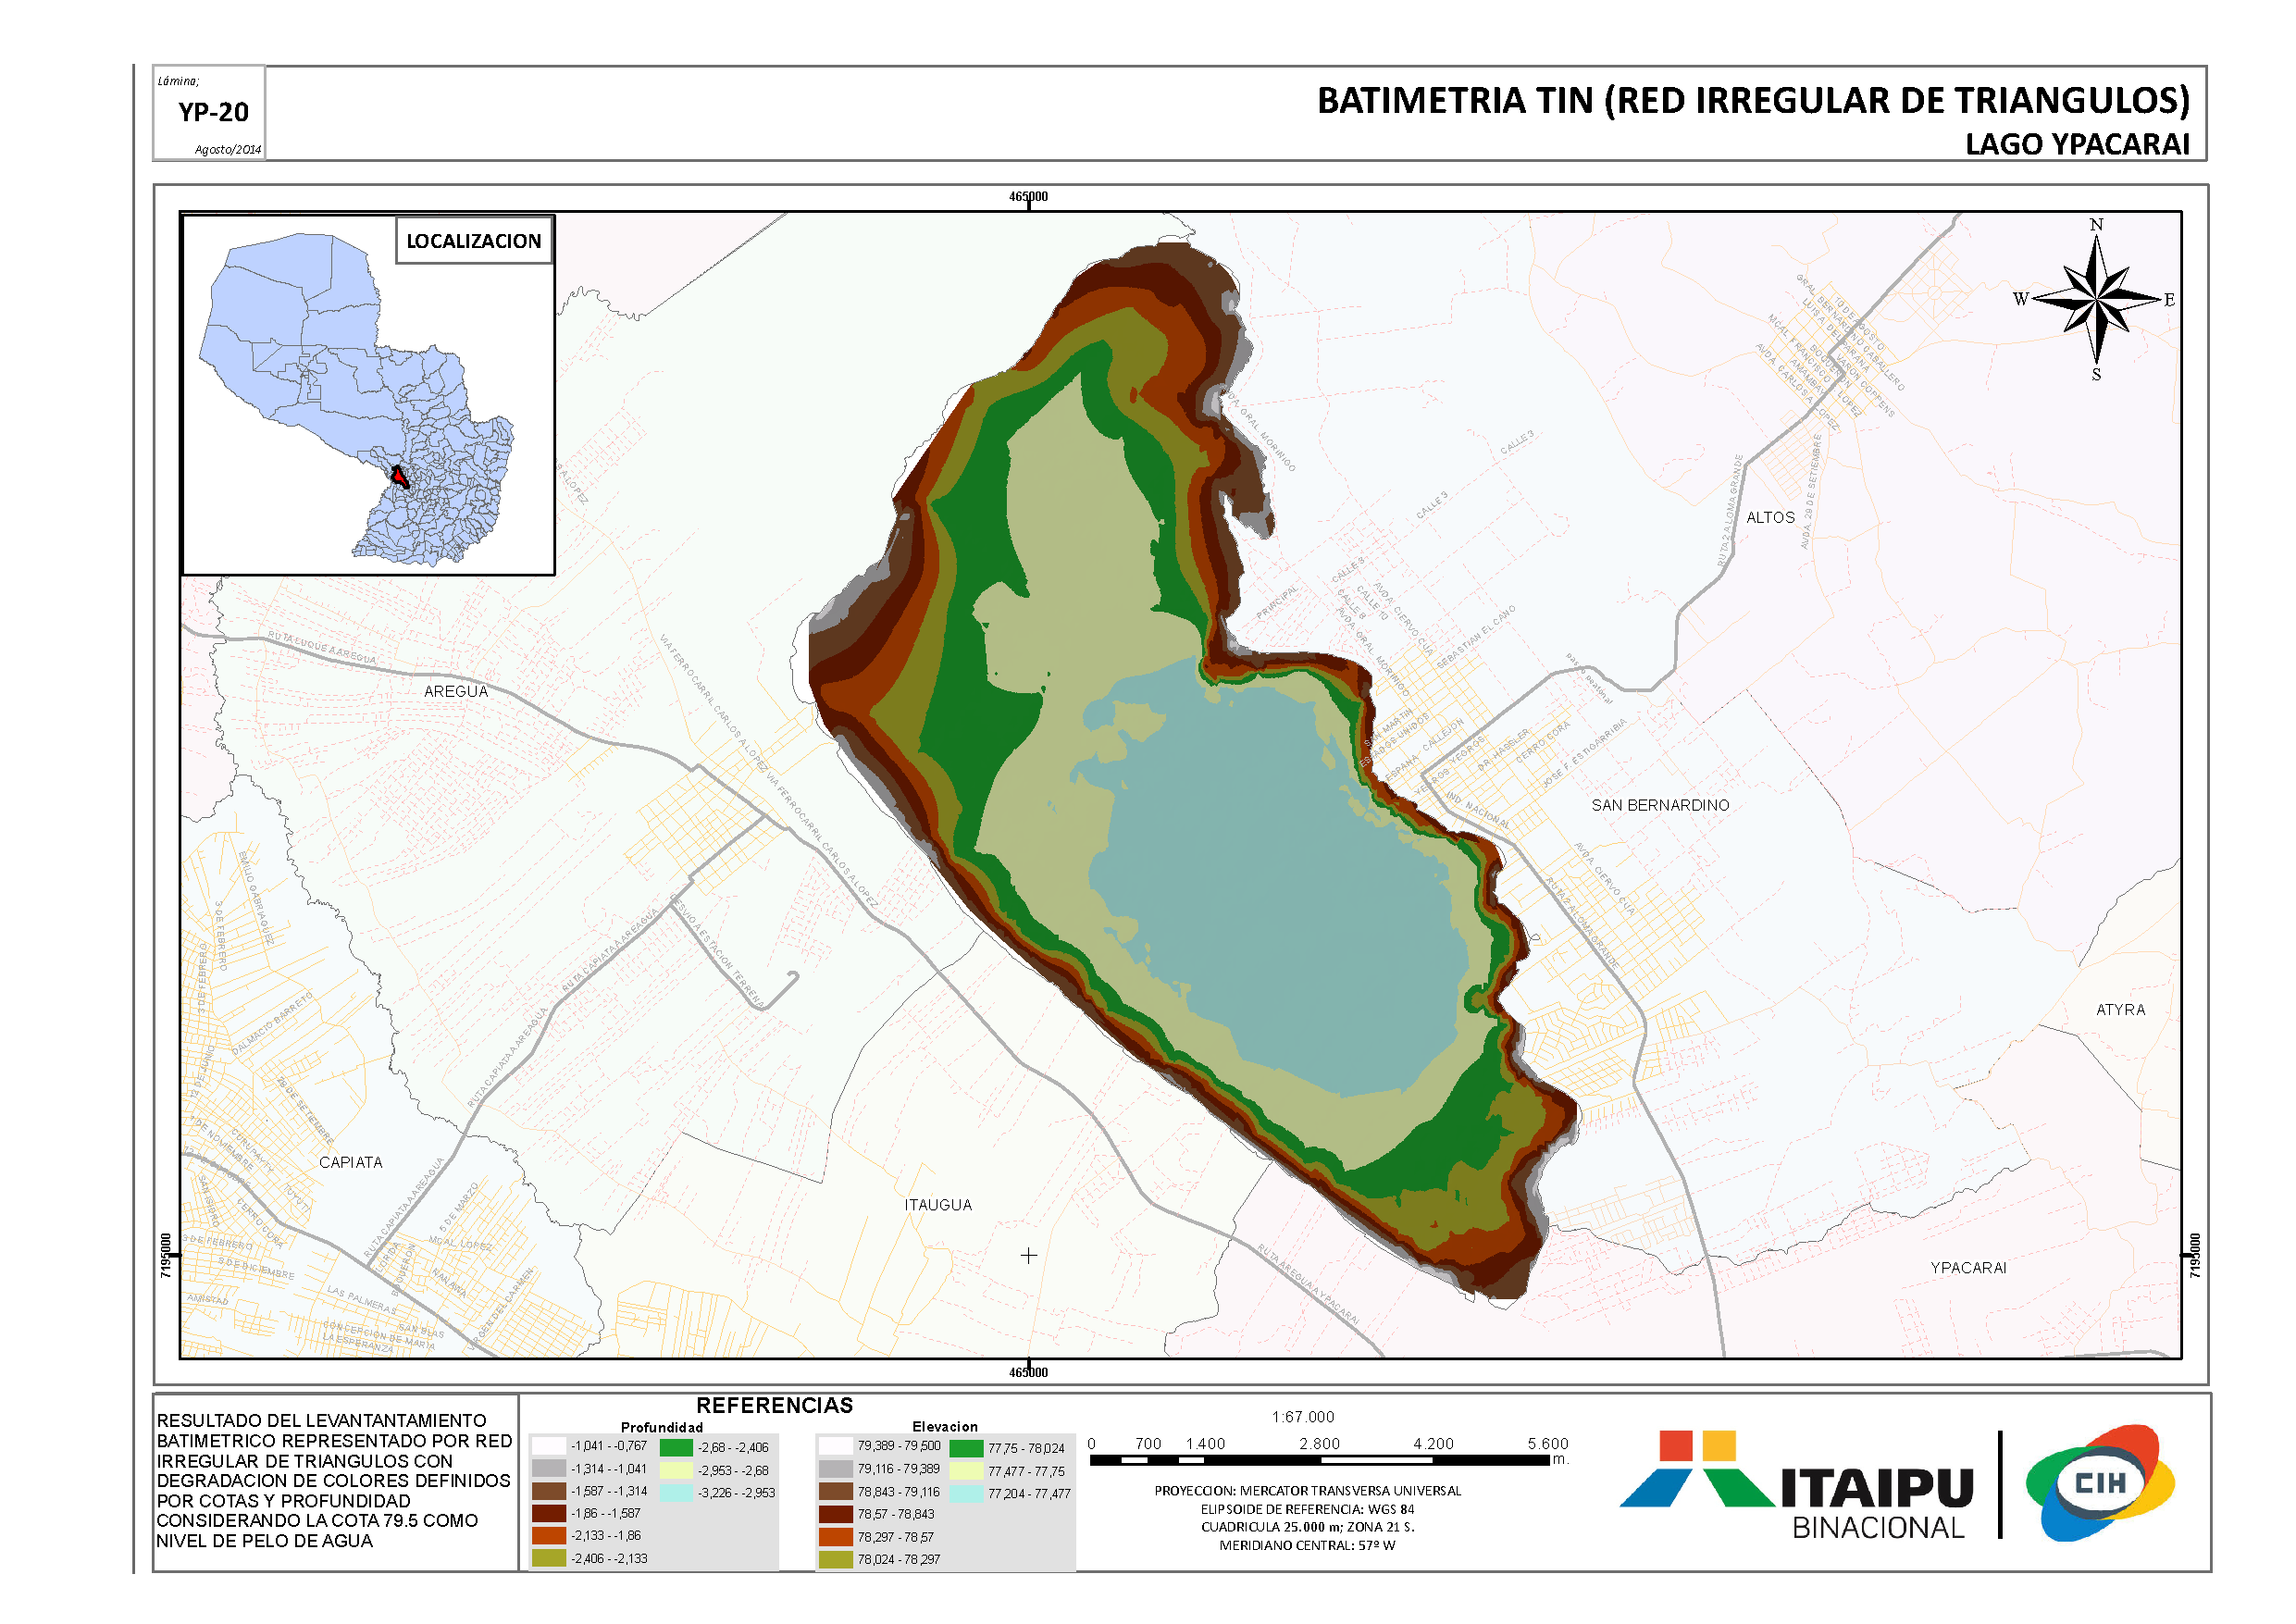
\includegraphics[width=150mm, height=100mm]{Imagenes/cap3/Batimetria_lago_Ypacarai_TIN_A3.pdf}
%     \caption[Batimetr\'ia lago Ypakarai]{Batimetr\'ia TIN (Red Irregular de triángulos), lago Ypakarai} \textbf{Fuente:}  Itaipu Binacional.
%     \label{fig:BatimetriaItaipu}
% \end{figure}

\chapter*{Anexo B: Cormor\'an - I}
\addcontentsline{loa}{appendix}{Anexo B: Cormor\'an -I }
\label{appendix: cormoran}
\setcounter{figure}{0}    

El diseño final de la sonda, fue el resultado de varias versiones que fueron modificándose de tal manera que resulte mejor y se adapte a los requerimientos del proyecto.
Partiendo de un diseño de un misil militar por su dise\~no din\'amico , similar al propuesto por [1], modificado hasta la versión final con el cual se realizaron las pruebas. Su diseño modular est\'a pensado para el caso que se le requiera sacar o añadir uno o m\'as sensores, se pueda seguir utilizando la sonda con cambios mínimos para adaptación.
La primera sonda fue impresa en su totalidad con una impresora 3D, en material Acrilonitrilo butadieno Estireno(ABS), por sus propiedades de alta resistencia al impacto y su baja degradación en presencia de líquidos. 
El diseño de la sonda (Sonda V4.3) utilizado en el Cormoran-I, esta disen\~ado para ser albergar a seis sensores específicos de la empresa Atlas Scientific.

\begin{itemize}
    \item Sonda PH de Plata/cloruro de plata de calidad científica, EZO pH Circuit.
    \item Sonda ORP de barra de platino, EZO OPR Circuit.
    \item Sonda de conductividad: 5 [\(\mu S/cm\)] a 200,000 [\(\mu S/cm\)], EZO Conductivity Circuit.
    \item EZO RGB, Sensor de color integrado 8 bit.
    \item Sonda de oxígeno disuelto, EZO OD Circuit.
    \item Sensor de Temperatura DS18B20. Sparkfun.
\end{itemize}
    
\section*{Versiones de la Sonda }
Se desarrollaron cuatro versiones de la sonda, con el programa de diseño CAD 3D SolidWorks 2015. La sonda es un ensamble de tres piezas principales, denominadas:

\begin{itemize}
\item \textbf{Frente} : Pieza frontal de la sonda, la función de esta pieza es principalmente de protección contra basura o objetos que puedan dañar a los sensores. Se dise\~no de forma cil\'indrica hueca de base circular para las versiones de la sonda Figura1-a y Figura1-b, las de base elipsoidal para las versiones Figura1-d y Figura1-e, Posee ranuras laterales para que el agua ingrese dentro de la cavidad hueca de esta pieza y los sensores puedan hacer las mediciones.  
\item \textbf{Anillo} : Pieza central de la sonda y enlace de las otras dos piezas, la función de esta pieza es servir de soporte a las sensores y posicionarlos de forma horizontal. En el caso que se requiera otros sensores, esta es la única pieza que tendría que ser adaptado a los nuevos sensores.
\item \textbf{Base}  : Pieza posterior de la sonda, su función es de protección de los cables de los sensores. 
\end{itemize}

\begin{enumerate}
\item \textbf{Sonda V0.0:} La versión inicial de la sonda, con diseño cilíndrico de base circular, el inconveniente principal de este diseño fue la debilidad estructural de la parte frontal de la sonda por la cantidad de ranuras, ademas el diseño de la punta dificultaba bastante para ser impreso en la impresora 3D.
\begin{figure}[ht]
    \centering
    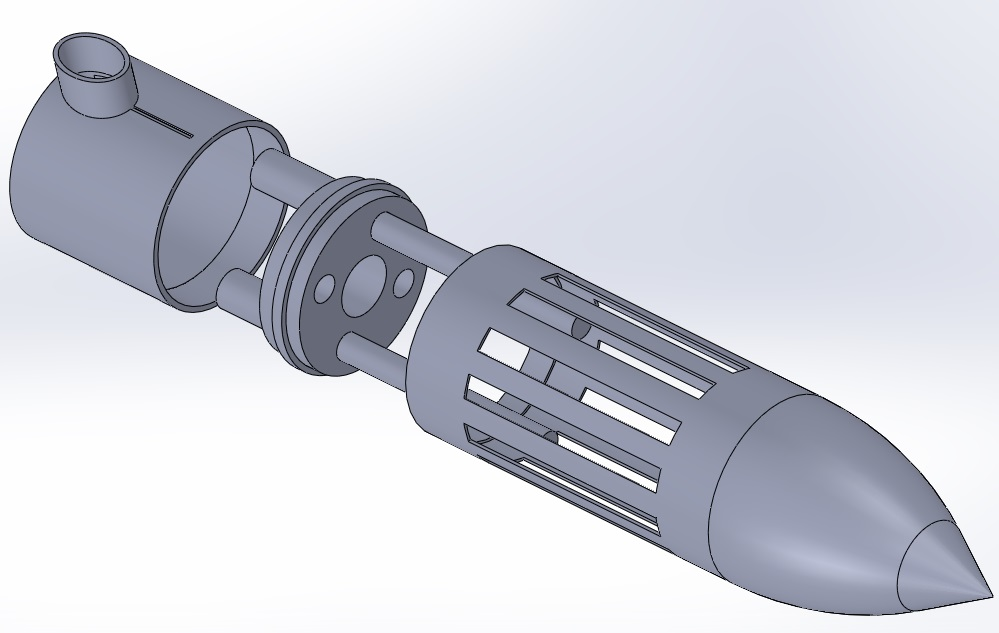
\includegraphics[width=50mm]{Imagenes/Sonda_v0.jpg}
    \caption{Caption}
    \label{fig:my_label}
\end{figure}

\item \textbf{Sonda V1.0:} La siguiente versión, resolvía los problemas de debilidad estructural de la parte frontal espaciando mas las ranuras y reemplazando la punta de la pieza frontal con un diseño mas redondeado para que pueda ser impresa con mayor facilidad.   
\item \textbf{Sonda V2.0:} En esta versión de la sonda, se probaron con otras geometrías para mejorar la dinámica del fluido, de esta forma cargar menos al motor propulsor del Dron. El inconveniente de este diseño fue, que por su geometría era mas grande que el anterior por tanto utilizaba mas material.
\item \textbf{Sonda V3.0:} La siguiente versión se opto por una base elipsoidal para la sonda, ademas se agrego al diseño un soporte para que pueda ser fijado al Dron con tornillos en la parte inferior, se realizaron cambios en la base para crear un ensamble mas dinámico. Fue la primera aproximación para el diseño final, el inconveniente de esta sonda era el soporte que resultaba poco practico de implementar y podría causar daños estructurales al casco del dron.
\item \textbf{Sonda V4.0:} La ultima versión resuelve el problemas de soporte, al agregar un riel en la parte superior de toda la sonda para fijarlo cuando se requiera al dron sin la utilización de tornillos o algún elemento fijador que pueda dañar el casco del dron.
\item \textbf{Sonda V4.1:} En la primera modificación de la versión 4 de la sonda, se optimizo el tamaño de la pieza frontal de la sonda,  para utilizar menos material y ofrecer mayor protección a las puntas de los sensores.
\item \textbf{Sonda V4.2:} En la segunda revisión de la versión 4, se re diseño la parte posterior de la sonda, para reemplazar el sistema modo inicial que conectar los sensores al dron, que en las versiones anteriores se encontraba en la parte superior, y como esta versión se diseña el riel, se opto por hacer por una perforación e la base para que por ella pueda conectarse al Dron.
\item \textbf{Sonda V4.3:} En la ultima revisión de la versión 4, se re diseña la pieza central de la sonda para agregarle un juego de juntas de gomas circulares, por los agujeros preparados para los sensores para de esta forma ejercer sobre ellos un mejor agarre, ademas se modifica la dimensión de sensor ubicado en la parte central de la pieza.
\end{enumerate}


\begin{figure}[htbp]
    \centering
 %   \subfigure[V0.0]{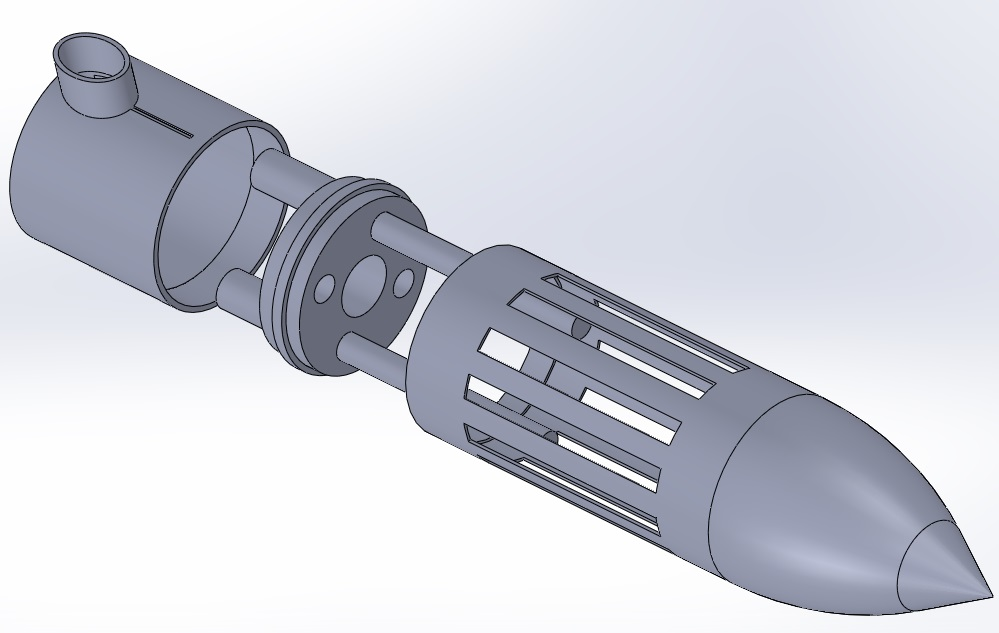
\includegraphics[width=50mm]{Imagenes/Sonda_v0.jpg}}
    
 %   \subfigure[V1.0]{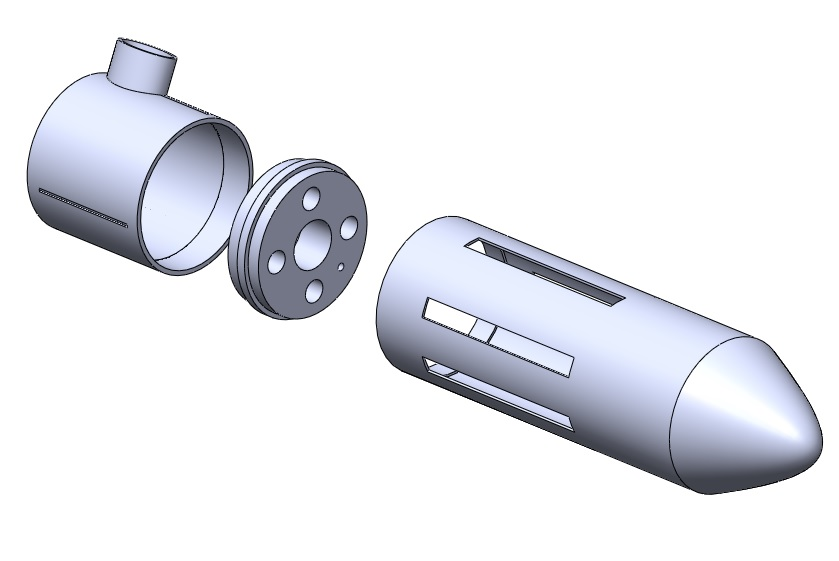
\includegraphics[width=50mm]{Imagenes/Sonda_v1.jpg}}
    
%    \subfigure[V2.0]{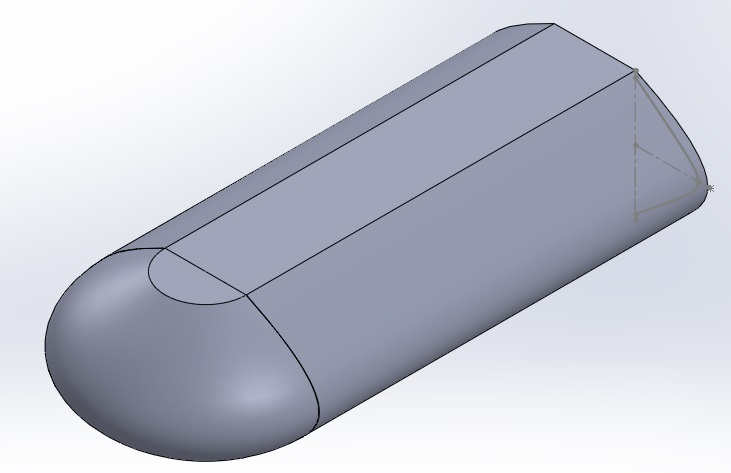
\includegraphics[width=50mm]{Imagenes/Sonda_v2.jpg}}
    
  %  \subfigure[V3.0]{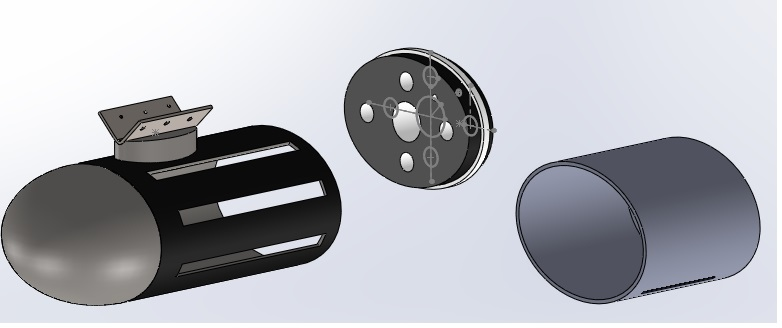
\includegraphics[width=50mm]{Imagenes/Sonda_v3.jpg}}
    
  %  \subfigure[V4.0]{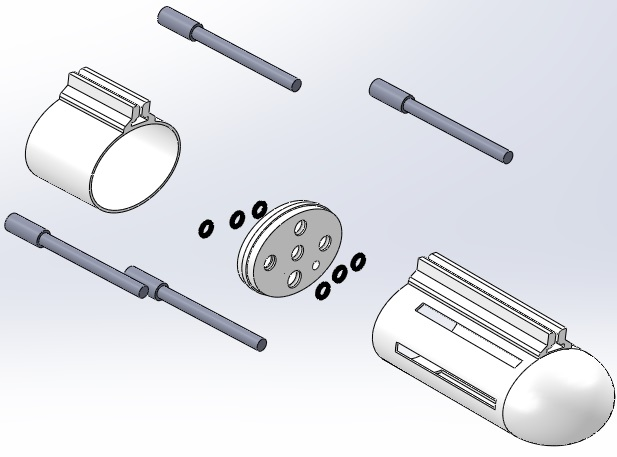
\includegraphics[width=50mm]{Imagenes/Sonda_v4.jpg}}
    
    \caption{Versiones Sonda. Fuente: elaboración propia} \label{fig:Sonda_Versiones1}
    \end{figure}
    
    \begin{figure}[htbp]
    \centering
%\subfigure[V4.3 . Frontal]{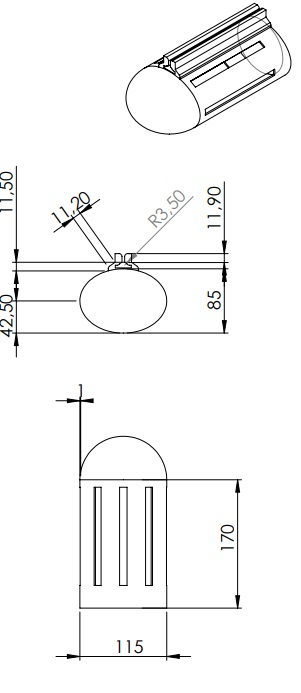
\includegraphics[width=40mm]{Imagenes/Sonda_v4_1.jpg}}
    
%    \subfigure[V4.3 . Anillo]{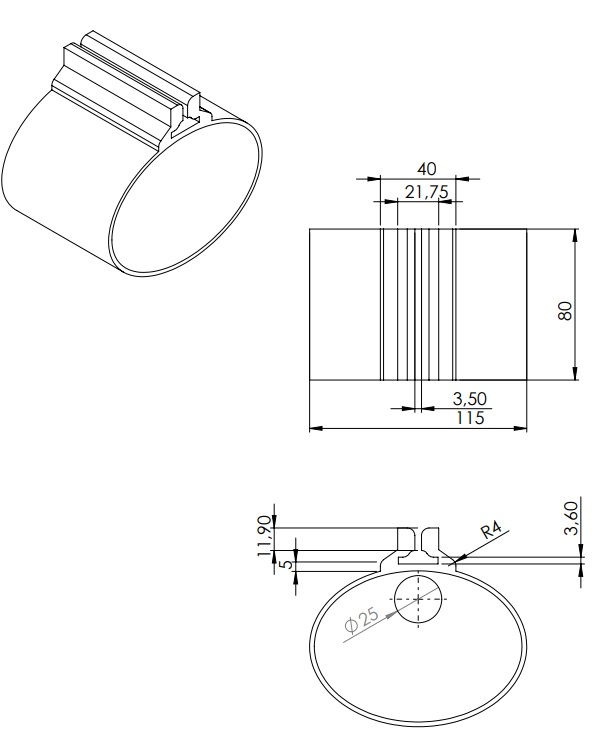
\includegraphics[width=40mm]{Imagenes/Sonda_v4_2.jpg}}
    
%    \subfigure[V4.3 . Base]{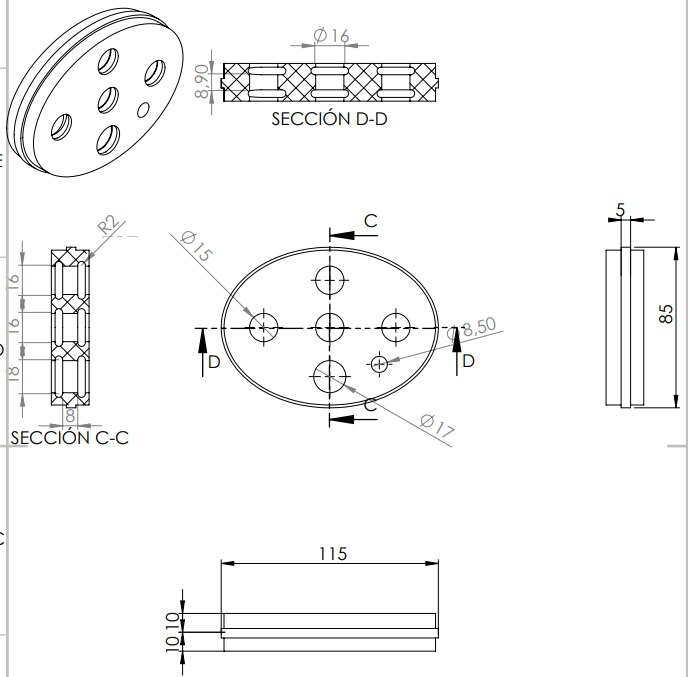
\includegraphics[width=40mm]{Imagenes/Sonda_v4_3.jpg}}
    
    \caption{Versiones Sonda. Fuente: elaboración propia} \label{fig:Sonda_Versiones2}
\end{figure}

\section*{Sonda v5.0}
Para el proyecto PINV15-177, se deberán realizar una serie de cambios al modelo final de la sonda utilizado en el CORMORAN-I, por la operación a multivinel, el material a ser utilizado y la ubicación de la electrónica.
\subsection*{Operación Multinivel}
Como se introduce la capacidad de poder censar a multiniveles, es necesario cambiar el tipo de material de construcción para que de esta forma se pueda sumergir con su propio peso, y no requiera de otro medio externo para sumergirse. 
\subsection*{Sonda Embebida}
Considerando que la versión 4.3, la sonda se fija por el casco del dron, el circuito de control y la base de datos se ubica dentro del dron, y los sensores de la sonda se conectan mediante cables coaxiales, segun datos proveídos por el informe de batimetria, realizado en el agosto del 2014  por la Dirección de Coordinación Ejecutiva del Centro Internacional de Hidroinformatica (CIH) dependiente de la Hidroeléctrica Itaipu, la máxima profundidad del lago Ypakarai es de 3,226[m], para la operación multinivel para estas profundidades la implementacion de versión actual resulta poco practica ya que se requerirán cables mas largos, expuestos al ambiente, agua, tracción pudiendo dañarse o registrar lecturas erróneas.\\ Para subsanar este inconveniente se propone que todo la electrónica se encuentre dentro de la sonda, en la parte posterior o base, de esta forma ademas eliminar el uso de cables, la sonda por si sola ya sera capaz de operar.

\subsection*{Primera Versi\'on sonda Embebida}

\subsection*{Diseño - Modelado}
El dise\~no y modelado de la sonda se realizo, utilizando el software de modelacion 3D SolidWorks.
El realizo el diseño de forma modular, de tal forma que que la sonda se adaptar con cambios mínimos en el caso de ser requerido, ante posibles cambios de configuración como ser, adición de otro sensor o modo de operación.    
La sonda consta de tres partes o módulos principales:

\begin{itemize}
\item \textbf{Base}: Modulo no reemplazable, a fabricarse en acero inoxidable, en esa sección de la sonda se almacenara toda la electrónica de control, procesamiento de señales provenientes de los sensores, alimentación y la base de datos de las lecturas registradas por los sensores. Este modulo debe de ser hermético 

\item \textbf{Anillo}: Modulo reemplazable, a ser fabricado de acero inoxidable, parte central de la sonda, la función de esta pieza es de mantener a los sensores posicionados correctamente y cumple la función de sello para la base, de esta forma cerrar de forma hermética la base.

\item \textbf{Envolvente}: Modulo reemplazable, a ser fabricado en material ácido poliláctico  láctico (PLA), la envolvente es un pieza que rodea todo la otros dos módulos, y su función principal es de proteger la parte frontal de los sensores y mejorar la dinámica del fluido mediante su geometría impreso totalmente en impresora 3D.  

\end{itemize}

\begin{figure}[ht]
\centering
\fbox{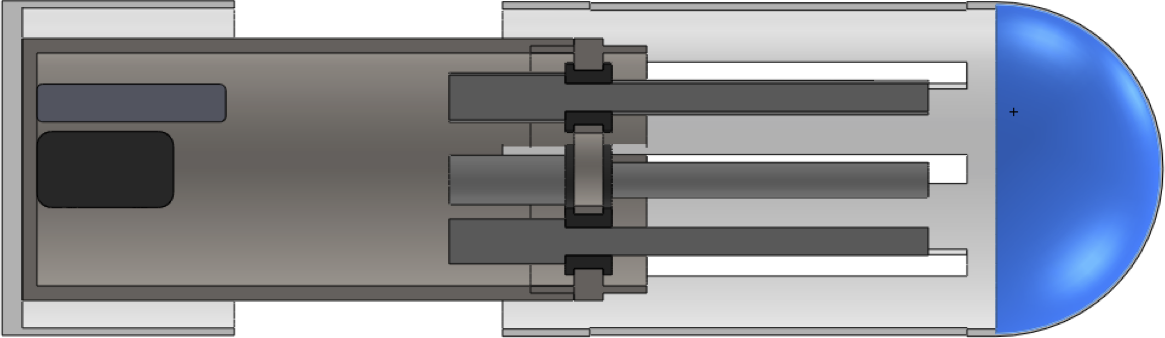
\includegraphics[scale=0.6]{Imagenes/2019/CompletoV5_0555.png} }
\caption{Dise\~no Sonda Completa. Fuente: elaboración propia}
\label{fig:SondaV5}
\end{figure}

\begin{figure}[ht]
\centering
\fbox{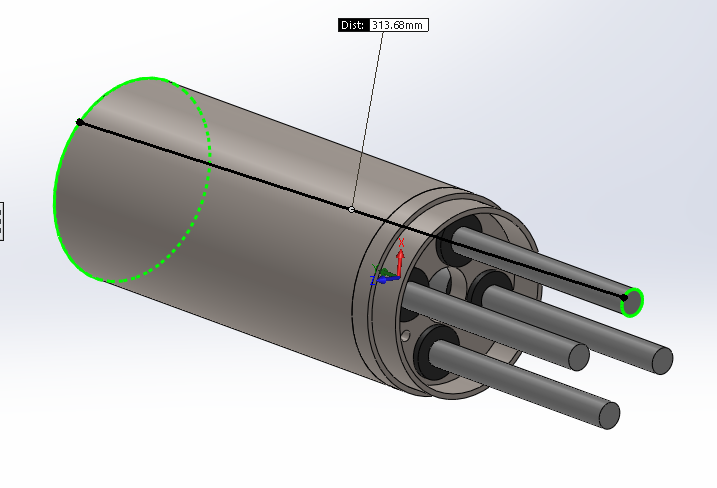
\includegraphics[scale=0.6]{Imagenes/2019/misilv5a.png} }
\caption{Dise\~no Base y anillo. Fuente: elaboración propia}
\label{fig:BaseAnilloV5}
\end{figure}

\section*{Sonda V6.0}
\subsection*{Diseño - Modificaciones}
Por la falta de materiales del dise\~no anterior 
se realizar\'on modif\'idicaciones para poder fabricar con materiales que s\'i pudimos conseguir en el pa\'is, 
en el diseño anterior estaba pensado fabricar la sonda en acero inoxidable.
El material utilizado fue Nylon que requiri\'o de un rediseño de la sonda conformada por dos elementos principales denominados base y anillo. 
\textbf{Base: }
Para una mejor robustez la base, se ensancharon las paredes internas y se dise\~no con  rosca interna Whitworth fina.\\ 
\begin{figure}[ht]
\centering
\fbox{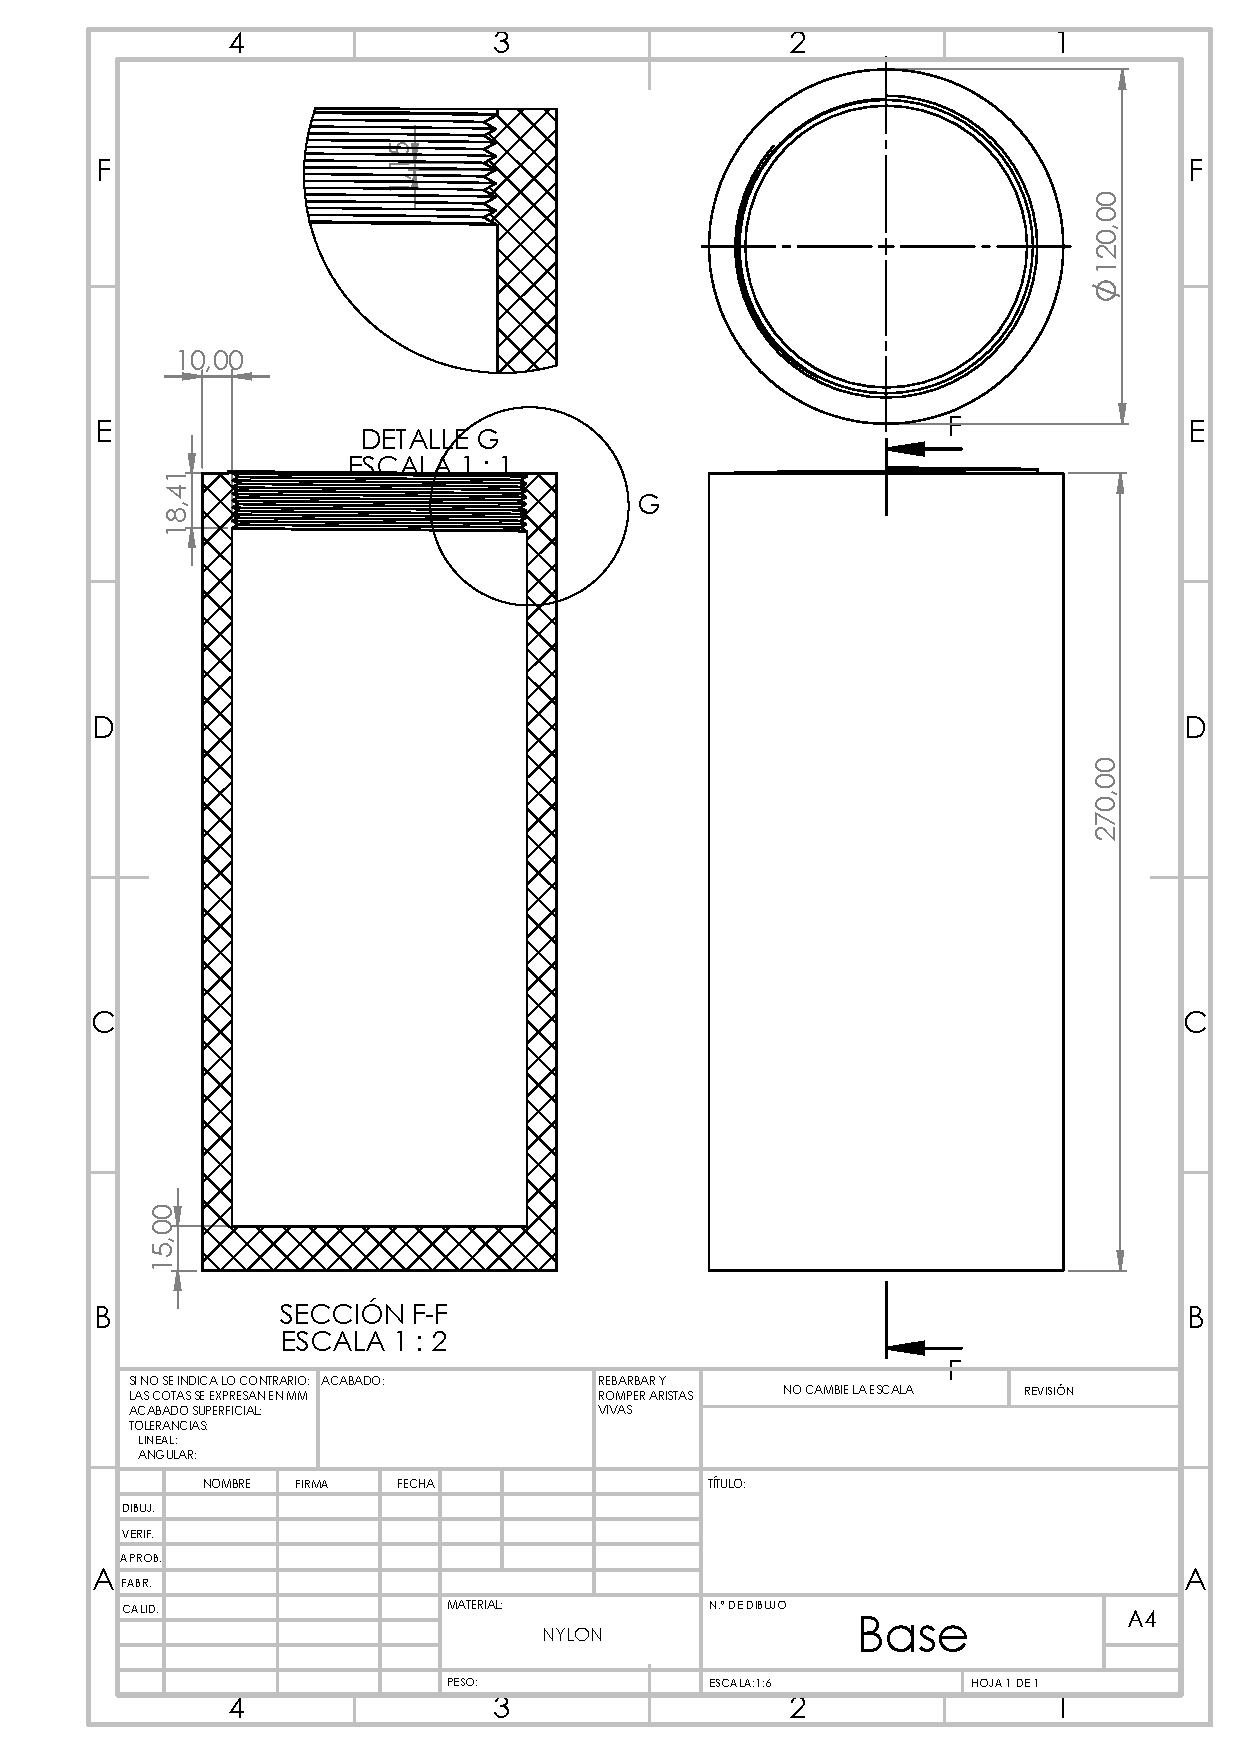
\includegraphics[scale=0.65]{Imagenes/2019/Base2019.PDF} }
\caption{Dise\~no final de la base. Fuente: elaboración propia}
\label{fig:Base2019}
\end{figure}

\textbf{Anillo: }
El diseño anterior Figura: \ref{fig:SondaV5}, se contemplaba el uso de O-ring para el sellado de la sonda, por las dificultades t\'ecnicas para la fabricaci\'on de las ranuras necesarias se opt\'o por otro dispositivo de sellado denominado,  reten hidr\'aulico, dos reten hidr\'aulico por abertura de cada sensor
\\
\begin{figure}[ht]
\centering
\fbox{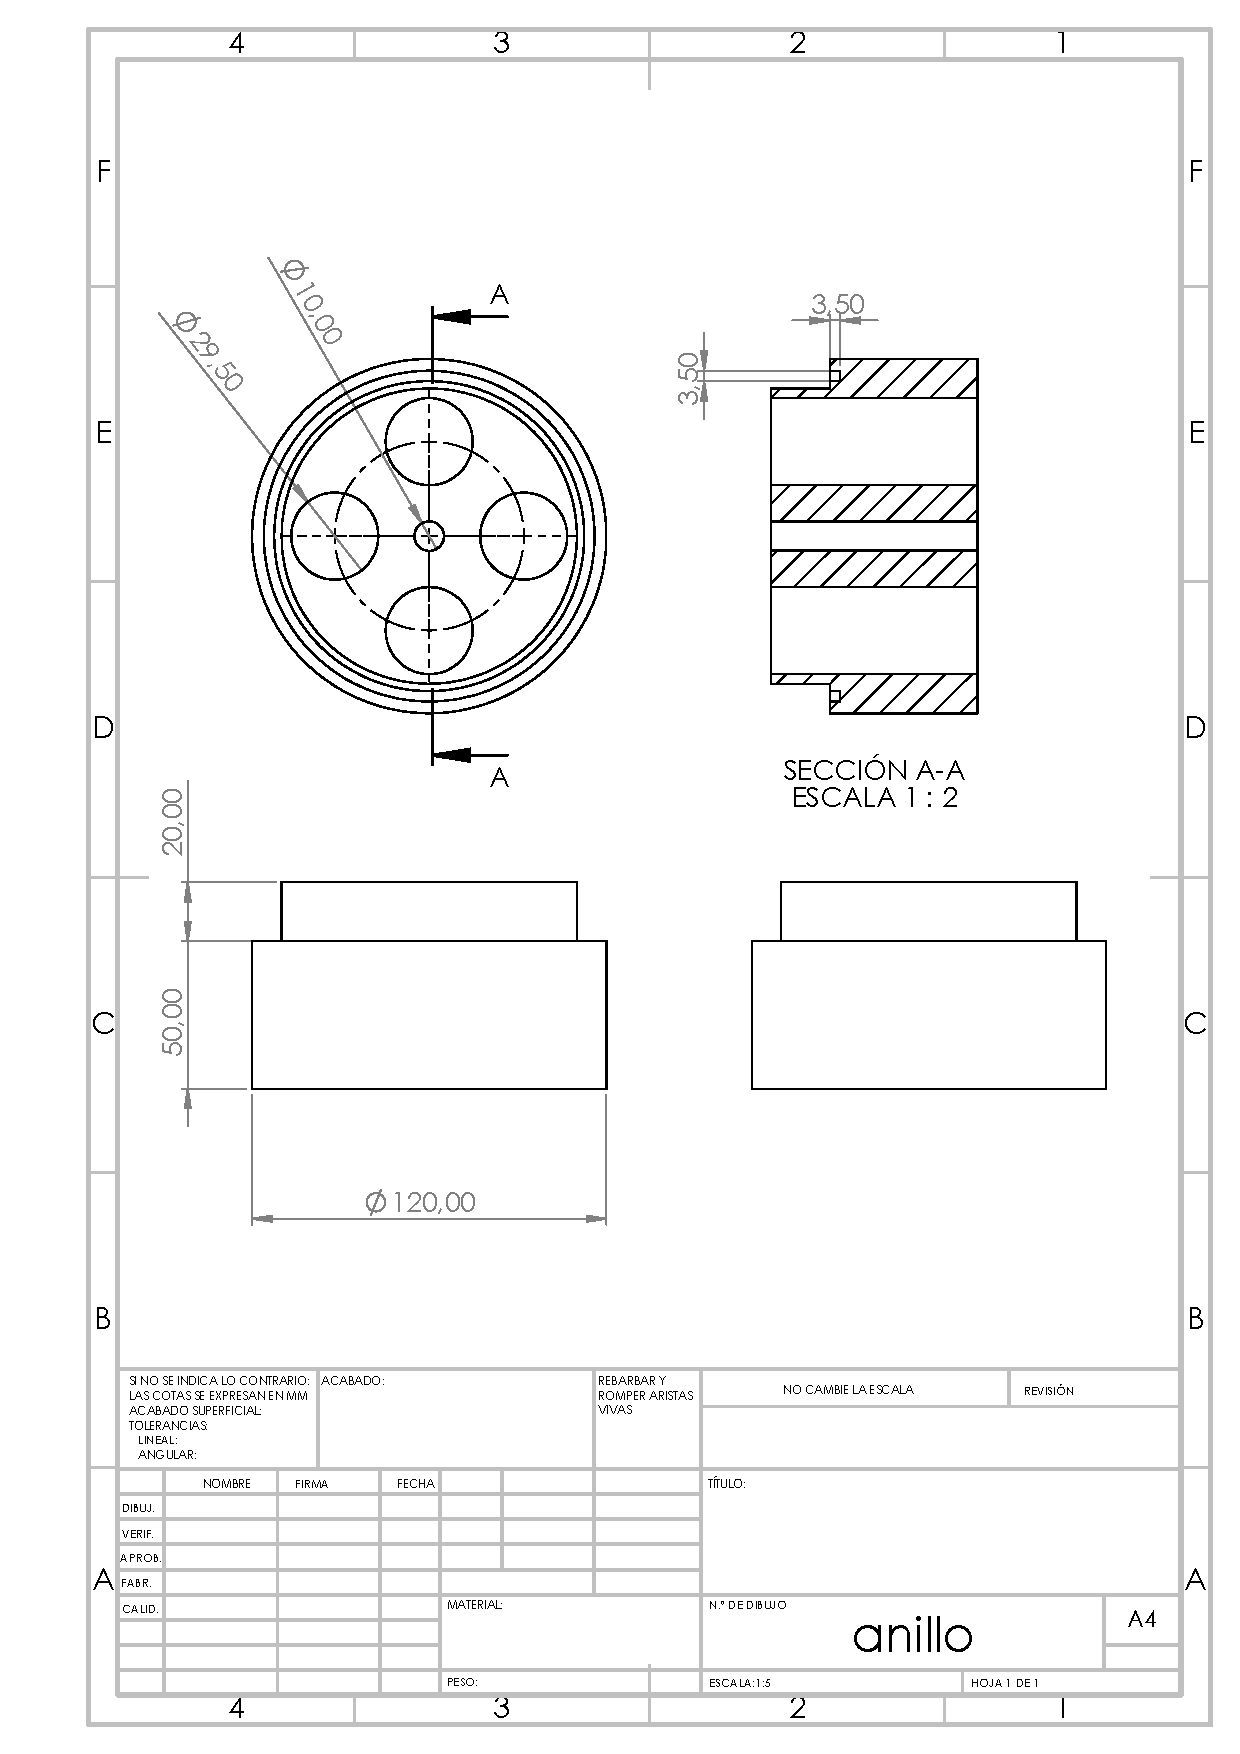
\includegraphics[scale=0.6]{Imagenes/2019/anillo2019.PDF} }
\caption{Dise\~no final del anillo. Fuente: elaboración propia}
\label{fig:Anillo2019_anexo}
\end{figure}

\chapter*{Anexo C}
\addcontentsline{loa}{appendix}{Anexo C: Esquematicos}
\label{appendix: c}
\setcounter{figure}{0}    

\begin{figure}[ht]
    \centering
    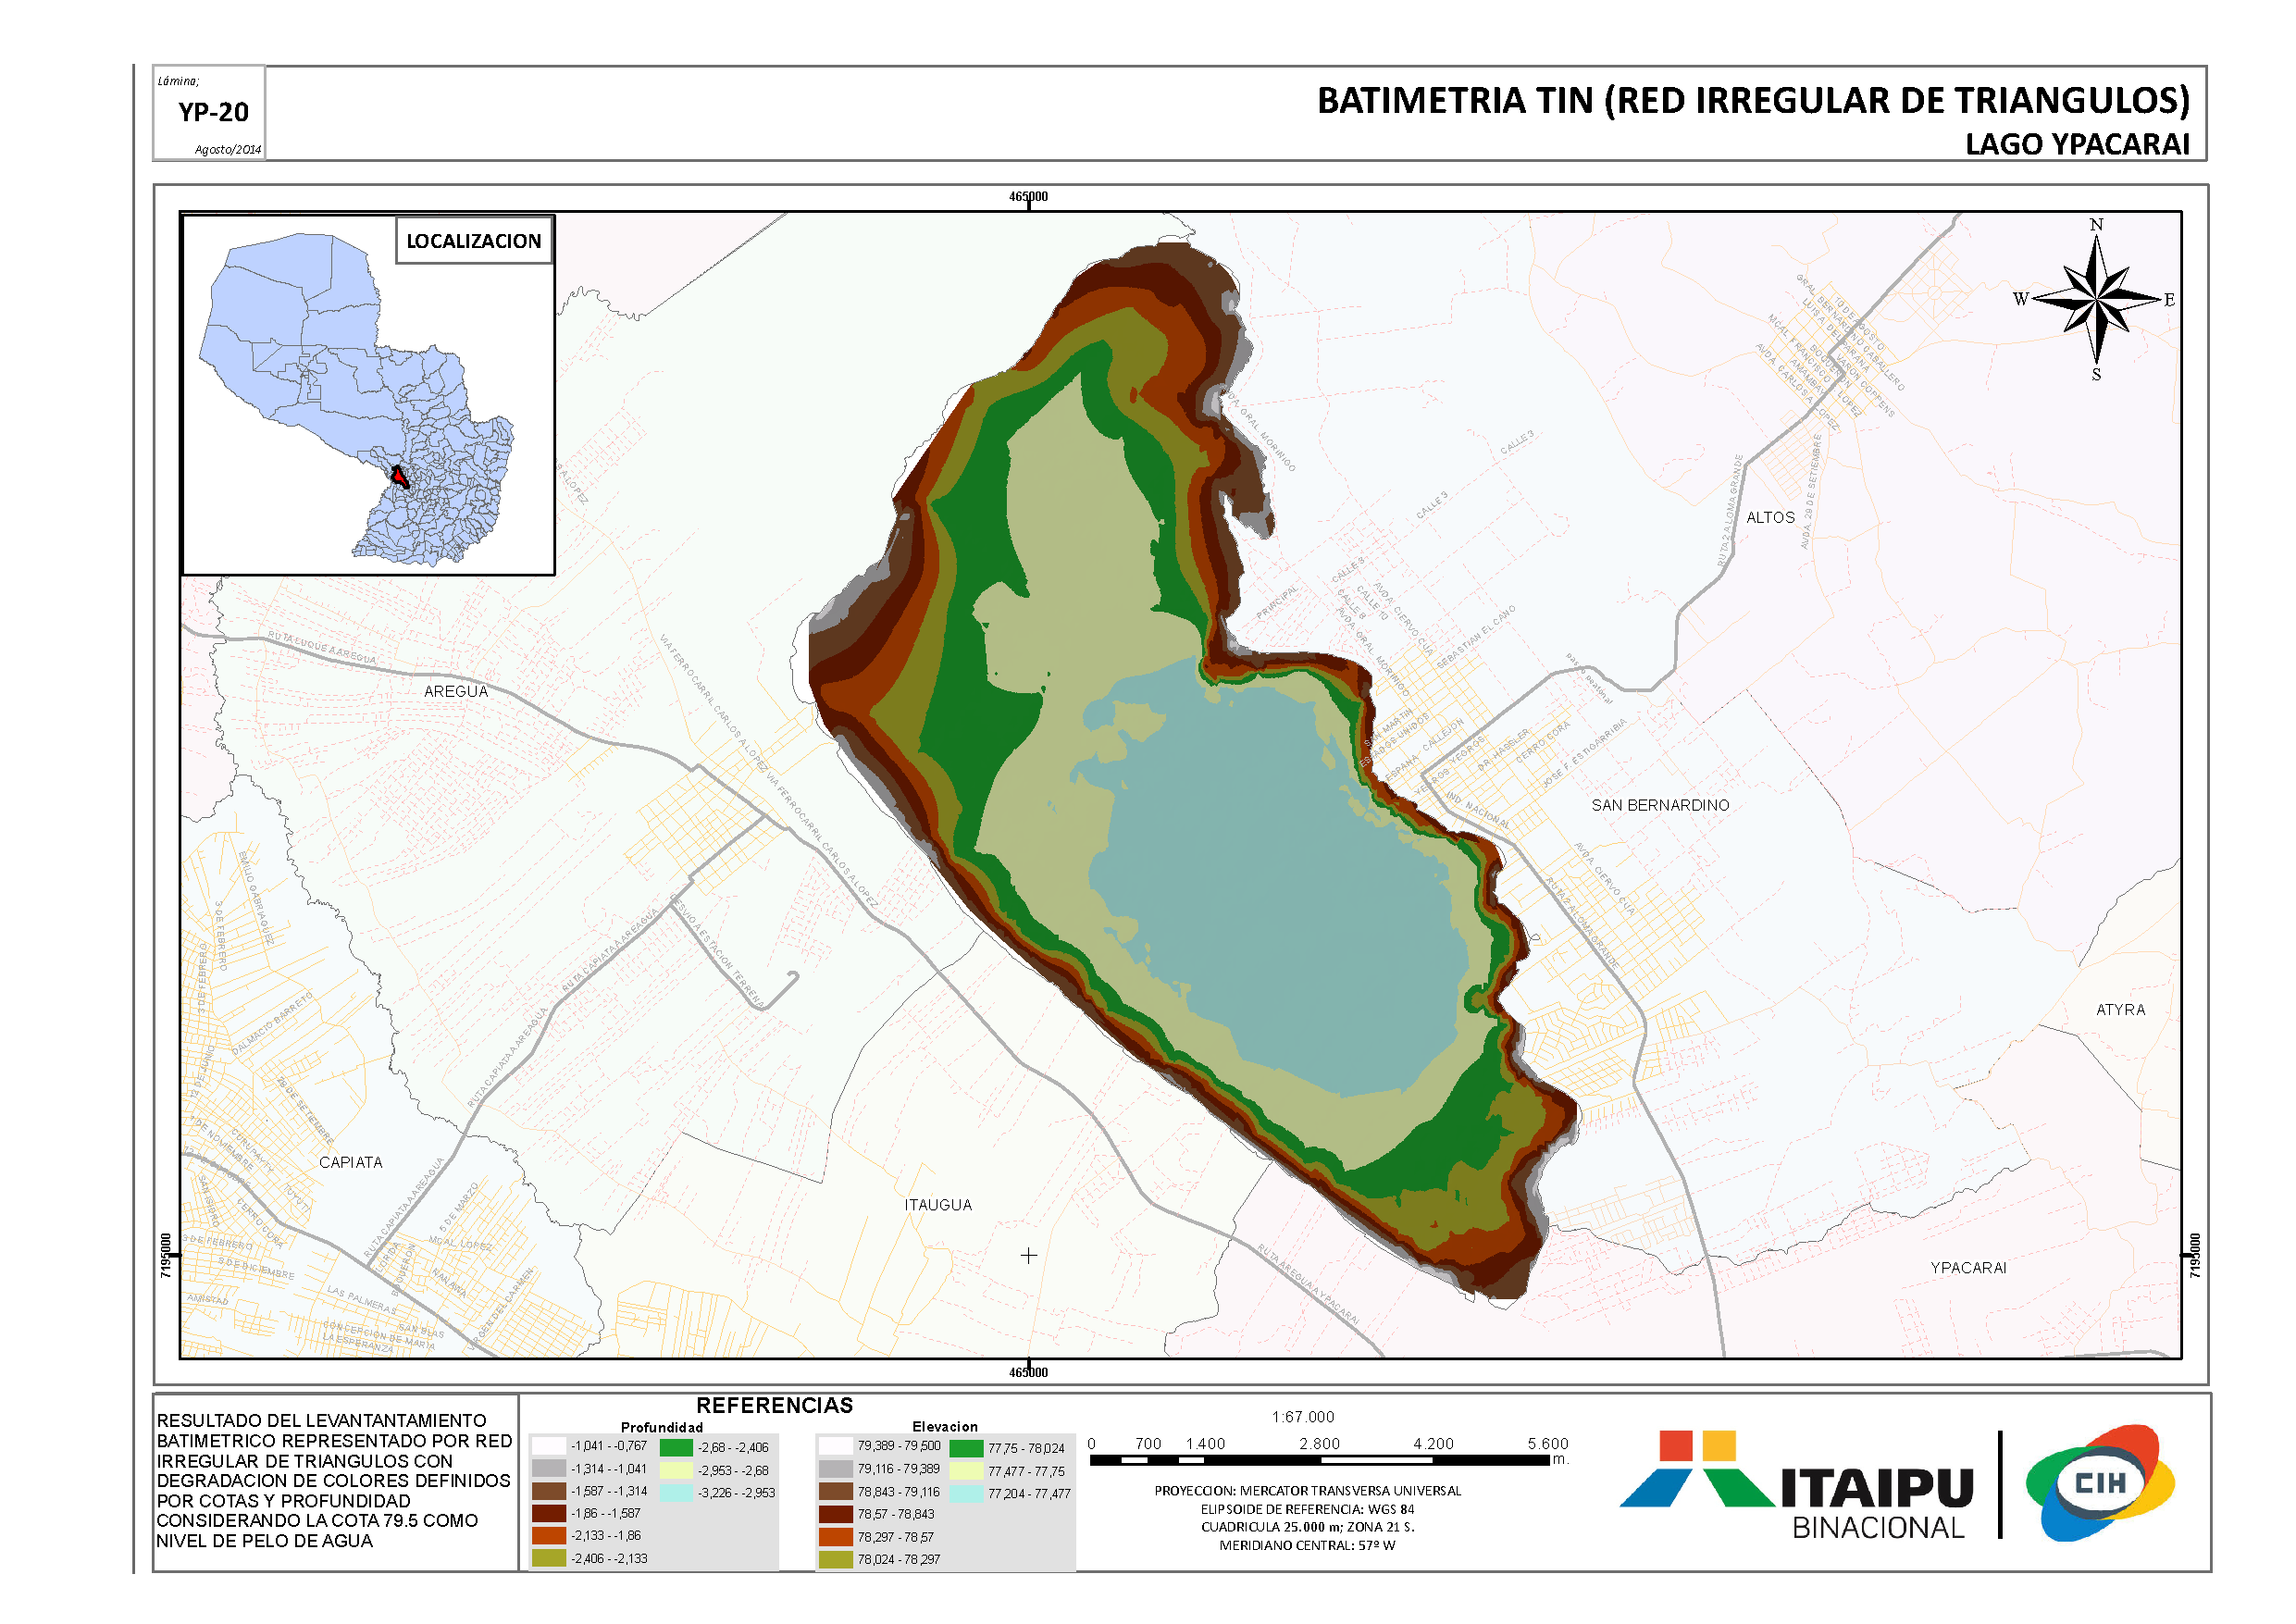
\includegraphics[width=150mm, height=100mm]{Imagenes/cap3/Batimetria_lago_Ypacarai_TIN_A3.pdf}
    \caption[BATIMETRIA TIN lago Ypakarai]{Batimetr\'ia TIN (RED IRREGULAR DE TRIANGULOS), lago Ypakarai} \textbf{Fuente: Itaipu Binacional.}
    \label{fig:ModuloFrontal}
\end{figure}

\chapter*{Anexo D: Poster}
\addcontentsline{loa}{appendix}{Anexo D: Divulgación Póster}
\label{appendix: poster}
\setcounter{figure}{0}    
\begin{figure}[ht]
    \centering
    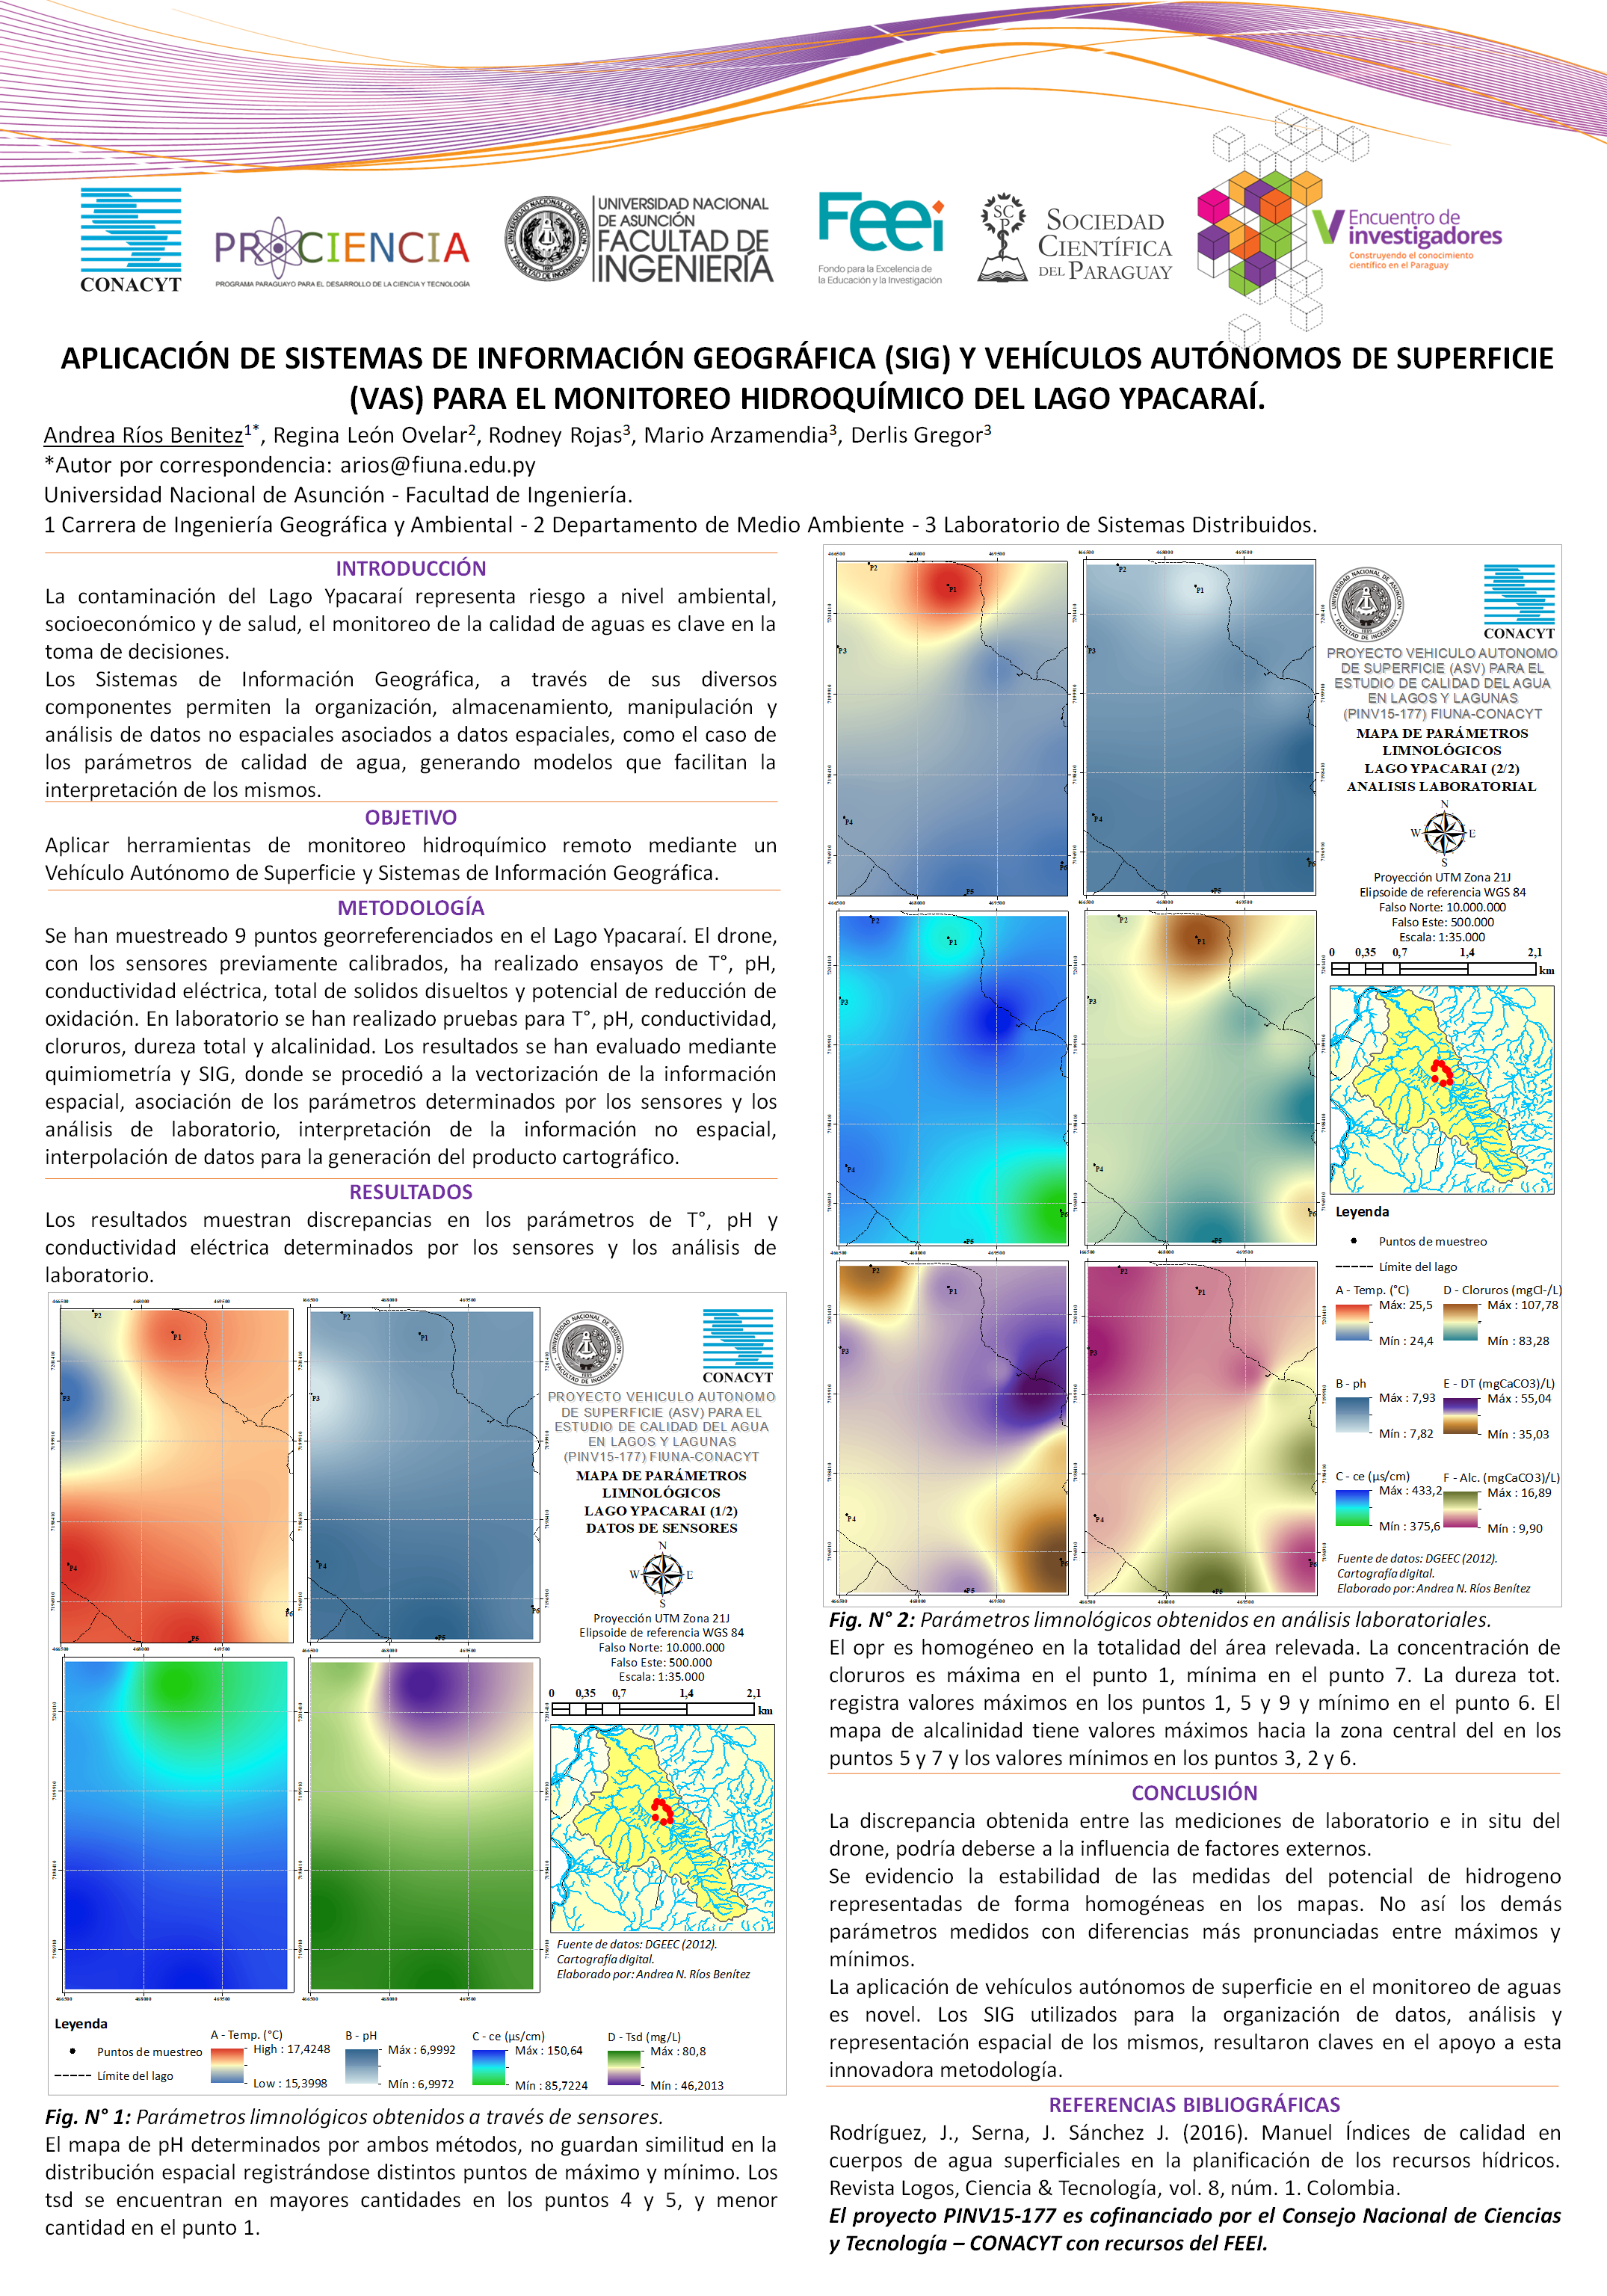
\includegraphics[width=0.78\textwidth]{Imagenes/cap5/poster-SIG-lago.png}
    \caption[Póster presentado en el V Encuentro de Investigadores 2020]{Póster presentado.}\textbf{Fuente:} \cite{noauthor_facultad_2020}
    \label{Fig:poster}
\end{figure}
% \end{appendices}

\chapter*{Anexo E: Diccionario de t\'opicos}
\addcontentsline{loa}{appendix}{Anexo E: Diccionario de t\'opicos}
\label{appendix: Topicos}
Los t\'opicos se construyeron considerando la ruta de comunicaci\'on e interacci\'on entre los distintos los componentes involucrados. Se estableci\'o como la ra\'iz principal la sonda por ser el elemento principal encargado de centralizar todas las comunicaciones entre todos los dispositivos.

\begin{itemize}
    \item \textbf{T\'opicos Banderas:} Los t\'opicos banderas se utilizan para verificar que los dispositivos est\'en disponibles. El script consulta en cada ciclo durante se requiera la comunicaci\'on con alg\'un componente.
    \begin{itemize}
        \item \textbf{sonda/sonar/flag}: bandera de verificaci\'on de conexi\'on con el subsistema de medici\'on de profundidad, retorna True cuando se solicita la confirmaci\'on de conexi\'on.
        \item \textbf{sonda/grua/flag}: bandera de verificaci\'on de conexi\'on con el subsistema de la g\'ua, retorna True cuando se solicita la confirmaci\'on de conexi\'on.
        \item \textbf{sonda/asv/flag}: bandera de verificaci\'on de conexi\'on con el subsistema ASB, retorna True cuando se solicita la confirmaci\'on de conexi\'on.
        \item \textbf{sonda/remoto/flag}: bandera de verificaci\'on de conexi\'on con el centro de monitoreo remoto, retorna True cuando se solicita la confirmaci\'on de conexi\'on.
        \item \textbf{sonda/muestreo/flag}: bandera de verificaci\'on de conexi\'on con los sensores, retorna True cuando se solicita la confirmaci\'on de conexi\'on y confirma adem\'as que los todos los sensores de la sonda están listos.
        \item \textbf{sonda/asv/monitoreo/inicio}: bandera utilizada para indicar el inicio del proceso de monitorio, una vez que le ASV se posicione en el lugar de medici\'on, env\'ia un TRUE para iniciar el proceso de muestreo.
        \item \textbf{sonda/asv/monitoreo/fin}: bandera de utilizada para indicar al ASV que puede avanzar al siguiente punto del mapa, una vez la sonda culmine su algoritmo de muestreo y almacene en su base de datos local, env\'ia un True al ASV para que se pueda desplazar al siguiente punto.


    \end{itemize}
    \item \textbf{T\'opicos recepci\'on de datos}: son t\'opicos que contienen datos espec\'ificos de cada uno de los subsistemas, que son necesarios para realizar alg\'un tipo de accion. 
        \begin{itemize}
        \item \textbf{sonda/sonar/cm}: Recibe el dato del subsistema de medici\'on de profundidad con la distancia sensada en ese instante, en formato string que luego se convierte en el formato float para mejor manejo. 
        \item \textbf{sonda/grua/status}:Bandera utilizada para indicar el inicio o fin de un tarea de descenso o ascenso, el estado por defecto es false y el estado de finalizaci\'on es true.
        \item \textbf{sonda/raspberry/PH}:Dato del sensor de pH, correspondiente a la lectura de muestreo de ph, el dato le\'do se env\'ia en formato string.
        \item \textbf{sonda/raspberry/temp}:Dato del sensor de temperatura (T), correspondiente a la lectura de muestreo de T, el dato le\'do se env\'ia en formato string.
        \item \textbf{sonda/raspberry/DO}:Dato del sensor de Oxigeno disuelto (DO), correspondiente a la lectura de muestreo de DO, el dato le\'do se env\'ia en formato string.
        \item \textbf{sonda/raspberry/CE}:Dato del sensor de conductividad el\'ectrica (CE), correspondiente a la lectura de muestreo de CE, el dato le\'do se env\'ia en formato string.
        \item \textbf{sonda/raspberry/OPR}:Dato del sensor de potencial oxido reducci\'on (OPR), correspondiente a la lectura de muestreo de OPR, el dato le\'do se env\'ia en formato string.
        \item \textbf{sonda/raspberry/TDS}:Dato del sensor de total de solidos disultos (TSD), correspondiente a la lectura de muestreo de TDS, el dato le\'do se env\'ia en formato string.
        \item \textbf{sonda/raspberry/S}:Dato del sensor de salinidad (S), correspondiente a la lectura de muestreo de S, el dato le\'do se env\'ia en formato string.
    \end{itemize}
    \item \textbf{T\'opicos env\'io de datos}:
        \begin{itemize}
        \item \textbf{sonda/remoto/sensores}: Contiene la informaci\'on de todos los sensores en formato json, reparado para ser recepcionado en la estacion remota para su posterior almacenamiento en base de datos. 
    \end{itemize}
    
\end{itemize}

% \chapter*{Anexo E: Datos Recolectados }
% \addcontentsline{loa}{appendix}{Anexo E: Datos Recolectados}
% \label{appendix: DataSet}

% \begin{longtable}{lrrrrrrll}
% \toprule
% {} &    temp &     ph &    od &      ce &  tds &    opr &       latitud &      longitud \\
% \midrule
% 0   &  17.062 &  6.997 &  7.82 &  139.40 &   75 & -287.4 &   -25.3080784 &   -57.3089882 \\
% 1   &  17.062 &  6.996 &  8.41 &  139.80 &   75 & -288.9 &   -25.3079363 &    -57.309062 \\
% 2   &  17.062 &  6.997 &  8.42 &  139.40 &   75 & -331.7 &   -25.3077949 &   -57.3091294 \\
% 3   &  17.062 &  6.994 &  8.34 &  140.00 &   75 & -329.7 &   -25.3076496 &   -57.3091906 \\
% 4   &  17.125 &  6.998 &  8.13 &  140.60 &   75 & -305.5 &   -25.3075126 &   -57.3092379 \\
% 5   &  17.125 &  6.998 &  8.01 &  137.40 &   74 & -321.2 &   -25.3073487 &   -57.3092779 \\
% 6   &  17.062 &  6.997 &  8.26 &  137.70 &   74 & -314.7 &   -25.3071899 &   -57.3093343 \\
% 7   &  17.062 &  6.998 &  8.34 &  139.70 &   75 & -322.6 &    -25.307028 &   -57.3093909 \\
% 8   &  17.500 &  6.996 &  7.65 &  145.50 &   78 & -293.7 &   -25.3006786 &   -57.3109259 \\
% 9   &  17.500 &  7.000 &  7.84 &  145.80 &   78 & -311.4 &   -25.3005373 &   -57.3109948 \\
% 10  &  17.500 &  6.999 &  8.07 &  145.60 &   78 & -269.1 &   -25.3003832 &   -57.3110784 \\
% 11  &  17.500 &  7.000 &  8.09 &  144.40 &   77 & -334.8 &   -25.3002643 &   -57.3111271 \\
% 12  &  17.437 &  7.001 &  7.81 &  144.90 &   78 & -324.7 &   -25.3001741 &   -57.3111679 \\
% 13  &  17.437 &  7.000 &  7.97 &  143.50 &   77 & -280.1 &   -25.3000903 &   -57.3112034 \\
% 14  &  17.312 &  7.000 &  8.14 &  142.80 &   77 & -315.8 &   -25.3000096 &    -57.311225 \\
% 15  &  17.250 &  6.999 &  8.18 &  142.90 &   77 & -288.0 &   -25.2998655 &    -57.311243 \\
% 16  &  17.250 &  7.001 &  8.36 &  142.30 &   76 & -298.6 &    -25.299787 &   -57.3112701 \\
% 17  &  17.187 &  6.999 &  7.81 &  141.80 &   76 & -311.4 &   -25.2997187 &   -57.3113168 \\
% 18  &  17.187 &  6.999 &  8.28 &  142.40 &   76 & -271.6 &   -25.2996572 &   -57.3113551 \\
% 19  &  17.187 &  7.000 &  7.95 &  143.40 &   77 & -325.5 &   -25.2995856 &   -57.3113996 \\
% 20  &  17.187 &  7.001 &  8.36 &  139.60 &   75 & -289.0 &   -25.2995138 &   -57.3114343 \\
% 21  &  17.187 &  6.998 &  8.29 &  142.70 &   77 & -328.0 &   -25.2994517 &   -57.3114666 \\
% 22  &  17.187 &  7.001 &  8.18 &  142.30 &   76 & -300.4 &   -25.2993899 &   -57.3114931 \\
% 23  &  17.187 &  6.999 &  7.74 &  142.40 &   76 & -340.8 &   -25.2993147 &   -57.3115249 \\
% 24  &  17.125 &  6.998 &  7.75 &  142.60 &   77 & -304.5 &   -25.2992427 &   -57.3115594 \\
% 25  &  17.125 &  6.997 &  8.08 &  142.10 &   76 & -318.6 &   -25.2991792 &   -57.3115939 \\
% 26  &  17.125 &  6.998 &  7.92 &  142.40 &   76 & -332.1 &   -25.2991171 &   -57.3116356 \\
% 27  &  17.125 &  6.999 &  8.40 &  142.70 &   77 & -288.9 &   -25.2990551 &   -57.3116927 \\
% 28  &  17.187 &  6.997 &  8.34 &  143.20 &   77 & -292.0 &   -25.2990002 &   -57.3117588 \\
% 29  &  17.125 &  7.000 &  7.92 &  142.80 &   77 & -340.9 &   -25.2989616 &   -57.3118297 \\
% 30  &  17.187 &  6.999 &  8.08 &  142.80 &   77 & -345.2 &   -25.2989097 &   -57.3119013 \\
% 31  &  17.187 &  6.997 &  7.91 &  142.80 &   77 & -275.7 &   -25.2988509 &   -57.3119684 \\
% 32  &  17.187 &  6.998 &  7.87 &  142.90 &   77 & -270.8 &   -25.2987946 &   -57.3120423 \\
% 33  &  17.125 &  6.999 &  7.66 &    0.00 &    0 & -301.4 &   -25.2987333 &   -57.3121511 \\
% 34  &  17.125 &  6.999 &  7.93 &  142.90 &   77 & -297.3 &   -25.2986874 &   -57.3122969 \\
% 35  &  17.125 &  6.999 &  8.26 &    0.00 &    0 & -298.8 &   -25.2986832 &   -57.3124548 \\
% 36  &  17.125 &  6.999 &  8.20 &  137.80 &   74 & -316.7 &   -25.2987265 &   -57.3126037 \\
% 37  &  17.125 &  6.997 &  7.71 &  141.60 &   76 & -343.3 &   -25.2987808 &   -57.3127662 \\
% 38  &  17.125 &  6.998 &  7.77 &  142.10 &   76 & -325.4 &   -25.2988165 &   -57.3129326 \\
% 39  &  17.062 &  6.998 &  8.03 &  141.60 &   76 & -310.5 &   -25.2988561 &   -57.3130825 \\
% 40  &  17.062 &  6.997 &  7.68 &  140.70 &   76 & -322.7 &   -25.2988853 &   -57.3132542 \\
% 41  &  17.000 &  6.996 &  8.21 &  140.20 &   75 & -297.7 &   -25.2989144 &   -57.3134189 \\
% 42  &  16.937 &  6.998 &  7.95 &  140.30 &   75 & -320.2 &   -25.2989609 &   -57.3135853 \\
% 43  &  16.937 &  6.996 &  8.08 &  140.20 &   75 & -286.5 &    -25.299011 &   -57.3137401 \\
% 44  &  16.937 &  6.998 &  7.88 &  140.00 &   75 & -288.9 &   -25.2990585 &   -57.3139104 \\
% 45  &  16.937 &  6.998 &  7.70 &  140.60 &   75 & -269.3 &     -25.29909 &   -57.3140649 \\
% 46  &  16.937 &  6.997 &  7.81 &  140.50 &   75 & -319.3 &   -25.2991246 &   -57.3142316 \\
% 47  &  16.937 &  6.999 &  8.05 &   99.51 &   53 & -276.2 &   -25.2991623 &   -57.3143829 \\
% 48  &  16.937 &  6.998 &  7.86 &  141.00 &   76 & -280.0 &    -25.299191 &   -57.3145439 \\
% 49  &  16.937 &  6.998 &  8.39 &  139.50 &   75 & -274.6 &   -25.2992196 &   -57.3147204 \\
% 50  &  16.937 &  6.997 &  8.42 &  139.70 &   75 & -301.2 &    -25.299253 &   -57.3149005 \\
% 51  &  16.875 &  6.998 &  8.18 &    0.00 &    0 & -310.3 &   -25.2992895 &   -57.3150639 \\
% 52  &  16.812 &  6.996 &  8.11 &  138.60 &   74 & -329.6 &   -25.2993223 &   -57.3152185 \\
% 53  &  16.812 &  6.996 &  8.27 &  138.50 &   74 & -341.7 &   -25.2993432 &   -57.3154071 \\
% 54  &  16.750 &  6.995 &  7.90 &  138.50 &   74 & -269.6 &   -25.2993638 &   -57.3155819 \\
% 55  &  16.750 &  6.996 &  8.21 &  134.70 &   72 & -337.3 &   -25.2993885 &     -57.31574 \\
% 56  &  16.687 &  6.998 &  8.25 &    0.00 &    0 & -297.2 &    -25.299406 &   -57.3159079 \\
% 57  &  16.687 &  6.997 &  8.17 &  137.20 &   74 & -343.6 &   -25.2994319 &   -57.3160611 \\
% 58  &  16.687 &  6.995 &  8.25 &  137.90 &   74 & -317.8 &   -25.2994599 &   -57.3162159 \\
% 59  &  16.687 &  6.993 &  8.38 &  138.20 &   74 & -304.6 &   -25.2994749 &   -57.3163757 \\
% 60  &  16.625 &  6.995 &  8.27 &  137.90 &   74 & -309.6 &   -25.2994909 &   -57.3165406 \\
% 61  &  16.687 &  6.995 &  7.70 &  138.50 &   74 & -319.9 &   -25.2995129 &   -57.3167027 \\
% 62  &  16.625 &  6.997 &  8.16 &  137.90 &   74 & -301.1 &   -25.2995479 &   -57.3168689 \\
% 63  &  16.625 &  6.997 &  8.20 &  136.20 &   73 & -280.0 &   -25.2995798 &   -57.3170282 \\
% 64  &  16.625 &  6.997 &  8.26 &  138.10 &   74 & -327.4 &   -25.2995945 &    -57.317193 \\
% 65  &  16.625 &  6.999 &  8.37 &  137.80 &   74 & -332.8 &   -25.2995799 &   -57.3173349 \\
% 66  &  16.625 &  6.998 &  7.76 &  136.90 &   73 & -279.3 &   -25.2995786 &   -57.3174981 \\
% 67  &  16.625 &  6.999 &  7.93 &  137.70 &   74 & -314.6 &   -25.2995776 &   -57.3176658 \\
% 68  &  16.562 &  6.997 &  8.10 &  137.60 &   74 & -296.7 &   -25.2995848 &   -57.3178324 \\
% 69  &  16.562 &  6.997 &  8.06 &  136.60 &   73 & -278.6 &   -25.2996079 &   -57.3180172 \\
% 70  &  16.562 &  6.998 &  7.78 &  134.50 &   72 & -279.5 &   -25.2996365 &   -57.3181762 \\
% 71  &  16.562 &  6.997 &  8.36 &  137.20 &   74 & -317.2 &   -25.2996721 &   -57.3183317 \\
% 72  &  16.562 &  6.997 &  7.82 &  137.10 &   74 & -295.8 &   -25.2997024 &   -57.3184763 \\
% 73  &  16.562 &  6.997 &  7.71 &  137.60 &   74 & -319.8 &   -25.2997378 &   -57.3186518 \\
% 74  &  16.500 &  6.997 &  7.77 &  136.80 &   73 & -325.9 &   -25.2997737 &   -57.3188114 \\
% 75  &  16.500 &  6.998 &  7.94 &  137.10 &   74 & -332.5 &   -25.2997894 &   -57.3189676 \\
% 76  &  16.500 &  6.998 &  7.82 &  136.20 &   73 & -314.6 &   -25.2997783 &   -57.3191374 \\
% 77  &  16.437 &  6.996 &  7.69 &  135.80 &   73 & -313.8 &   -25.2997586 &   -57.3193089 \\
% 78  &  16.375 &  6.998 &  7.96 &  135.80 &   73 & -330.9 &   -25.2997348 &   -57.3194466 \\
% 79  &  16.312 &  6.996 &  7.86 &  135.10 &   72 & -311.3 &    -25.299729 &   -57.3195957 \\
% 80  &  16.312 &  6.997 &  7.96 &  135.90 &   73 & -294.6 &   -25.2997361 &   -57.3197495 \\
% 81  &  16.250 &  6.998 &  7.98 &  135.40 &   73 & -286.9 &   -25.2997595 &   -57.3199135 \\
% 82  &  16.250 &  6.999 &  8.26 &  134.80 &   72 & -335.5 &    -25.299769 &   -57.3200742 \\
% 83  &  16.250 &  6.997 &  8.09 &  135.10 &   72 & -307.4 &   -25.2997519 &   -57.3202329 \\
% 84  &  16.250 &  6.998 &  7.82 &  134.30 &   72 & -329.3 &   -25.2997354 &   -57.3203789 \\
% 85  &  16.250 &  6.999 &  8.29 &  134.50 &   72 & -300.4 &   -25.2997272 &   -57.3205222 \\
% 86  &  16.187 &  6.997 &  8.15 &  134.80 &   72 & -334.8 &   -25.2996895 &   -57.3206751 \\
% 87  &  16.187 &  6.998 &  7.94 &  134.30 &   72 & -286.2 &   -25.2996367 &   -57.3208252 \\
% 88  &  16.187 &  6.998 &  8.34 &  125.60 &   67 & -320.5 &   -25.2995847 &    -57.320957 \\
% 89  &  16.125 &  6.997 &  8.42 &  131.10 &   70 & -304.5 &   -25.2995391 &   -57.3211186 \\
% 90  &  16.125 &  6.996 &  7.78 &  132.40 &   71 & -316.9 &   -25.2995059 &   -57.3212758 \\
% 91  &  16.062 &  6.999 &  7.85 &  133.40 &   72 & -336.7 &   -25.2994807 &   -57.3214437 \\
% 92  &  16.062 &  6.998 &  8.03 &  112.60 &   60 & -286.1 &   -25.2994562 &   -57.3216007 \\
% 93  &  16.062 &  6.996 &  8.37 &  134.00 &   72 & -301.5 &   -25.2994241 &   -57.3217572 \\
% 94  &  16.062 &  6.997 &  8.16 &  133.60 &   72 & -326.4 &    -25.299378 &   -57.3219091 \\
% 95  &  16.062 &  6.997 &  8.40 &  133.80 &   72 & -296.7 &     -25.29934 &   -57.3220626 \\
% 96  &  16.000 &  6.997 &  7.72 &  133.80 &   72 & -331.8 &   -25.2992888 &   -57.3222236 \\
% 97  &  16.062 &  6.996 &  7.85 &  133.90 &   72 & -335.8 &   -25.2992494 &   -57.3223777 \\
% 98  &  16.062 &  6.996 &  8.30 &  133.80 &   72 & -285.0 &    -25.299196 &   -57.3225293 \\
% 99  &  16.062 &  6.996 &  7.74 &  127.80 &   69 & -310.8 &   -25.2991432 &   -57.3226766 \\
% 100 &  16.062 &  6.997 &  8.06 &  134.10 &   72 & -280.7 &   -25.2990914 &   -57.3228306 \\
% 101 &  16.000 &  6.996 &  8.20 &  133.40 &   72 & -295.2 &   -25.2990507 &   -57.3229867 \\
% 102 &  15.937 &  6.996 &  7.97 &  133.10 &   71 & -278.2 &   -25.2990138 &   -57.3231502 \\
% 103 &  15.937 &  6.998 &  8.40 &  133.70 &   72 & -277.8 &    -25.298971 &   -57.3233059 \\
% 104 &  15.937 &  6.996 &  7.80 &  133.50 &   72 & -333.5 &   -25.2989395 &   -57.3234658 \\
% 105 &  15.937 &  6.995 &  7.70 &  132.80 &   71 & -302.8 &    -25.298891 &   -57.3236139 \\
% 106 &  15.875 &  6.996 &  8.29 &  133.60 &   72 & -286.3 &   -25.2988329 &   -57.3237553 \\
% 107 &  15.875 &  6.996 &  7.92 &  133.00 &   71 & -322.9 &    -25.298774 &   -57.3238926 \\
% 108 &  15.875 &  6.996 &  7.97 &  134.40 &   72 & -280.4 &   -25.2987155 &   -57.3240414 \\
% 109 &  15.875 &  6.996 &  7.74 &  134.20 &   72 & -288.0 &   -25.2986423 &   -57.3242028 \\
% 110 &  15.875 &  6.996 &  8.06 &   18.13 &    9 & -342.1 &   -25.2985696 &   -57.3243265 \\
% 111 &  16.187 &  6.998 &  7.87 &   10.84 &    5 & -316.7 &   -25.2984867 &   -57.3244587 \\
% 112 &  16.687 &  6.997 &  7.68 &    4.62 &    2 & -270.2 &   -25.2984081 &    -57.324579 \\
% 113 &  17.000 &  6.997 &  8.19 &    0.00 &    0 & -285.8 &   -25.2983234 &   -57.3247004 \\
% 114 &  17.375 &  6.995 &  7.77 &  135.80 &   73 & -333.8 &   -25.2982206 &   -57.3248257 \\
% 115 &  16.687 &  6.997 &  7.72 &  135.10 &   73 & -306.2 &   -25.2981215 &   -57.3249228 \\
% 116 &  16.312 &  6.997 &  8.30 &  135.30 &   73 & -311.5 &   -25.2980165 &    -57.325019 \\
% 117 &  16.125 &  6.997 &  8.02 &  136.00 &   73 & -313.8 &   -25.2979072 &    -57.325117 \\
% 118 &  16.125 &  6.997 &  7.90 &  136.30 &   73 & -323.9 &   -25.2978025 &   -57.3252129 \\
% 119 &  16.125 &  6.993 &  8.36 &  137.70 &   74 & -338.6 &   -25.2977033 &   -57.3252869 \\
% 120 &  16.187 &  6.995 &  7.97 &  139.50 &   75 & -323.0 &   -25.2976014 &   -57.3253769 \\
% 121 &  16.312 &  6.996 &  8.38 &  140.50 &   75 & -341.1 &   -25.2974875 &    -57.325468 \\
% 122 &  16.437 &  6.995 &  8.36 &  141.80 &   76 & -309.4 &   -25.2973792 &   -57.3255437 \\
% 123 &  16.562 &  6.997 &  8.23 &  143.50 &   77 & -327.4 &   -25.2972699 &   -57.3256089 \\
% 124 &  16.750 &  6.998 &  7.71 &  144.90 &   78 & -299.2 &   -25.2971574 &   -57.3256609 \\
% 125 &  16.875 &  6.998 &  7.91 &  145.80 &   78 & -309.7 &   -25.2970594 &   -57.3257134 \\
% 126 &  17.000 &  6.996 &  8.27 &  146.30 &   79 & -301.6 &   -25.2969424 &   -57.3257742 \\
% 127 &  17.062 &  6.998 &  7.80 &  147.80 &   79 & -271.8 &   -25.2968309 &   -57.3258298 \\
% 128 &  17.187 &  6.998 &  8.28 &  142.40 &   76 & -305.3 &   -25.2967172 &   -57.3258898 \\
% 129 &  17.250 &  6.996 &  8.26 &  148.50 &   80 & -343.9 &   -25.2966067 &   -57.3259467 \\
% 130 &  17.375 &  6.997 &  7.89 &  150.50 &   81 & -344.2 &   -25.2964879 &   -57.3260024 \\
% 131 &  17.437 &  6.998 &  8.15 &  151.50 &   81 & -337.1 &   -25.2963842 &   -57.3260601 \\
% 132 &  17.562 &  6.997 &  8.15 &  151.70 &   81 & -291.7 &   -25.2962787 &    -57.326098 \\
% 133 &  17.687 &  6.997 &  8.07 &  145.30 &   78 & -290.3 &   -25.2961567 &   -57.3261287 \\
% 134 &  17.812 &  6.995 &  7.98 &  154.10 &   83 & -288.7 &   -25.2960395 &   -57.3261643 \\
% 135 &  17.875 &  6.996 &  7.73 &  154.40 &   83 & -311.5 &   -25.2959209 &   -57.3261977 \\
% 136 &  17.937 &  6.995 &  7.91 &  153.80 &   83 & -277.2 &   -25.2958022 &   -57.3262316 \\
% 137 &  17.937 &  6.996 &  8.24 &    0.00 &    0 & -333.5 &    -25.295693 &    -57.326272 \\
% 138 &  17.937 &  6.996 &  8.24 &  148.50 &   80 & -324.0 &   -25.2955831 &   -57.3263075 \\
% 139 &  17.875 &  6.995 &  8.17 &    0.00 &    0 & -341.6 &   -25.2954776 &   -57.3263306 \\
% 140 &  17.687 &  6.998 &  7.98 &   76.24 &   41 & -327.3 &   -25.2954019 &   -57.3263938 \\
% 141 &  17.312 &  6.997 &  8.17 &  143.00 &   77 & -271.1 &   -25.2953215 &   -57.3264807 \\
% 142 &  17.062 &  6.996 &  8.23 &  140.70 &   76 & -293.9 &   -25.2952508 &    -57.326556 \\
% 143 &  16.750 &  6.998 &  7.77 &  136.80 &   73 & -329.1 &   -25.2952003 &   -57.3266341 \\
% 144 &  16.750 &  6.997 &  7.74 &  133.10 &   71 & -291.2 &   -25.2951476 &   -57.3267138 \\
% 145 &  16.125 &  6.998 &  8.06 &  134.20 &   72 & -340.2 &   -25.2950987 &   -57.3268021 \\
% 146 &  15.937 &  6.999 &  7.84 &  132.80 &   71 & -307.2 &   -25.2950525 &   -57.3268648 \\
% 147 &  15.812 &  6.999 &  7.67 &  133.10 &   71 & -320.5 &   -25.2950078 &    -57.326931 \\
% 148 &  15.812 &  6.997 &  8.20 &  132.60 &   71 & -327.9 &   -25.2949628 &    -57.327009 \\
% 149 &  15.750 &  6.997 &  8.18 &  133.30 &   72 & -306.2 &   -25.2949146 &   -57.3270878 \\
% 150 &  15.687 &  7.000 &  8.18 &  133.50 &   72 & -333.5 &   -25.2948776 &    -57.327178 \\
% 151 &  15.687 &  6.998 &  7.79 &  133.20 &   71 & -291.1 &   -25.2948565 &   -57.3272805 \\
% 152 &  15.687 &  6.998 &  8.31 &  133.40 &   72 & -327.5 &   -25.2948416 &   -57.3273771 \\
% 153 &  15.625 &  7.001 &  8.19 &  134.50 &   72 & -338.7 &   -25.2948199 &   -57.3274839 \\
% 154 &  15.687 &  6.998 &  7.90 &  134.40 &   72 & -311.5 &   -25.2948125 &   -57.3275866 \\
% 155 &  15.687 &  6.999 &  8.13 &  133.90 &   72 & -295.5 &   -25.2947941 &   -57.3276904 \\
% 156 &  15.687 &  6.997 &  8.35 &  135.00 &   72 & -288.9 &   -25.2947657 &   -57.3277714 \\
% 157 &  15.687 &  6.998 &  7.83 &  134.80 &   72 & -333.2 &   -25.2947498 &   -57.3278572 \\
% 158 &  15.750 &  6.997 &  7.72 &  134.50 &   72 & -333.4 &   -25.2947266 &   -57.3279418 \\
% 159 &  15.750 &  6.998 &  7.78 &  134.00 &   72 & -276.5 &   -25.2946842 &   -57.3280127 \\
% 160 &  15.812 &  6.999 &  8.31 &  133.20 &   71 & -310.7 &   -25.2946406 &   -57.3281082 \\
% 161 &  15.812 &  6.999 &  7.79 &  133.60 &   72 & -323.2 &   -25.2946255 &   -57.3282104 \\
% 162 &  15.812 &  6.998 &  8.20 &  134.10 &   72 & -329.9 &      -25.2946 &   -57.3283004 \\
% 163 &  15.812 &  6.999 &  8.22 &  134.00 &   72 & -304.5 &   -25.2945797 &   -57.3283863 \\
% 164 &  15.812 &  6.997 &  7.69 &  134.30 &   72 & -288.9 &   -25.2945496 &   -57.3284707 \\
% 165 &  15.750 &  7.001 &  8.12 &  134.10 &   72 & -336.8 &   -25.2945301 &   -57.3285522 \\
% 166 &  15.812 &  7.001 &  8.27 &    0.00 &    0 & -317.6 &   -25.2945364 &   -57.3286482 \\
% 167 &  15.750 &  6.998 &  8.13 &  135.40 &   73 & -331.6 &   -25.2945543 &   -57.3287381 \\
% 168 &  15.812 &  7.000 &  8.24 &  135.50 &   73 & -286.3 &   -25.2946056 &   -57.3288189 \\
% 169 &  15.812 &  6.999 &  7.88 &  132.70 &   71 & -288.2 &   -25.2946677 &   -57.3288806 \\
% 170 &  15.875 &  6.999 &  8.12 &  134.70 &   72 & -342.9 &   -25.2947455 &   -57.3289288 \\
% 171 &  15.812 &  6.997 &  8.36 &  134.70 &   72 & -326.8 &   -25.2948377 &    -57.328955 \\
% 172 &  15.812 &  7.000 &  7.71 &  135.30 &   73 & -345.7 &   -25.2949306 &   -57.3289671 \\
% 173 &  15.812 &  6.997 &  7.81 &  134.80 &   72 & -338.3 &   -25.2950442 &   -57.3289681 \\
% 174 &  15.812 &  6.998 &  8.24 &  131.50 &   71 & -310.9 &   -25.2951541 &   -57.3289862 \\
% 175 &  15.812 &  6.999 &  8.10 &  134.90 &   72 & -329.4 &   -25.2952854 &   -57.3289943 \\
% 176 &  15.812 &  6.998 &  8.35 &  128.50 &   69 & -282.3 &   -25.2953969 &   -57.3289828 \\
% 177 &  15.812 &  6.997 &  8.11 &  135.30 &   73 & -320.5 &   -25.2954964 &   -57.3289573 \\
% 178 &  15.812 &  6.997 &  8.30 &  135.10 &   72 & -309.2 &   -25.2956019 &   -57.3289386 \\
% 179 &  15.812 &  6.998 &  7.68 &  135.50 &   73 & -343.6 &    -25.295723 &   -57.3289328 \\
% 180 &  15.812 &  6.998 &  8.33 &  135.30 &   73 & -320.6 &   -25.2958561 &   -57.3289559 \\
% 181 &  15.812 &  7.000 &  8.20 &  135.80 &   73 & -341.1 &   -25.2959829 &   -57.3289789 \\
% 182 &  15.812 &  6.999 &  7.76 &  135.10 &   72 & -303.1 &   -25.2961007 &   -57.3290236 \\
% 183 &  15.812 &  6.999 &  8.42 &  128.80 &   69 & -290.8 &   -25.2962202 &   -57.3290839 \\
% 184 &  15.812 &  6.997 &  8.11 &  135.90 &   73 & -271.3 &   -25.2963448 &   -57.3291246 \\
% 185 &  15.812 &  7.000 &  8.41 &  136.00 &   73 & -335.7 &   -25.2964478 &   -57.3291676 \\
% 186 &  15.875 &  6.999 &  7.99 &  136.70 &   73 & -273.5 &   -25.2965718 &   -57.3292094 \\
% 187 &  15.875 &  7.000 &  7.86 &  135.40 &   73 & -308.2 &   -25.2966928 &   -57.3292546 \\
% 188 &  15.937 &  6.999 &  8.25 &  137.00 &   74 & -328.3 &   -25.2968207 &   -57.3292848 \\
% 189 &  15.937 &  6.999 &  8.22 &  137.60 &   74 & -308.3 &   -25.2969472 &   -57.3293136 \\
% 190 &  15.937 &  6.999 &  7.96 &  137.50 &   74 & -331.3 &   -25.2970697 &   -57.3293626 \\
% 191 &  16.000 &  6.998 &  7.80 &  138.80 &   75 & -292.2 &     -25.29719 &   -57.3294072 \\
% 192 &  16.062 &  6.998 &  8.16 &  139.20 &   75 & -283.7 &   -25.2973056 &   -57.3294503 \\
% 193 &  16.125 &  6.998 &  8.07 &  136.50 &   73 & -273.9 &   -25.2974338 &   -57.3295137 \\
% 194 &  16.125 &  6.999 &  7.82 &  137.90 &   74 & -289.6 &    -25.297536 &   -57.3295718 \\
% 195 &  16.125 &  7.000 &  8.28 &  138.60 &   74 & -328.3 &   -25.2976733 &   -57.3296279 \\
% 196 &  16.125 &  6.999 &  7.70 &  138.40 &   74 & -271.5 &   -25.2977884 &   -57.3296864 \\
% 197 &  16.187 &  6.997 &  8.26 &  138.80 &   74 & -322.3 &   -25.2979142 &   -57.3297241 \\
% 198 &  16.187 &  6.999 &  7.78 &  138.00 &   74 & -280.4 &   -25.2980407 &   -57.3297634 \\
% 199 &  16.187 &  6.998 &  7.81 &  135.20 &   73 & -307.6 &   -25.2981485 &   -57.3298097 \\
% 200 &  16.187 &  6.997 &  8.11 &  137.00 &   73 & -323.5 &   -25.2982735 &   -57.3298502 \\
% 201 &  16.125 &  6.998 &  7.82 &  136.40 &   73 & -291.5 &   -25.2983951 &   -57.3299044 \\
% 202 &  16.125 &  6.995 &  8.42 &  134.40 &   72 & -296.3 &   -25.2985188 &   -57.3299527 \\
% 203 &  15.937 &  6.996 &  8.14 &  133.70 &   72 & -345.2 &   -25.2986436 &   -57.3299966 \\
% 204 &  15.937 &  6.998 &  8.39 &  133.30 &   72 & -340.4 &   -25.2987667 &    -57.330035 \\
% 205 &  15.875 &  6.997 &  7.89 &  132.30 &   71 & -271.8 &   -25.2988751 &   -57.3300672 \\
% 206 &  15.875 &  6.996 &  8.15 &  133.00 &   71 & -342.5 &   -25.2989943 &   -57.3300961 \\
% 207 &  15.875 &  6.998 &  7.86 &  133.30 &   71 & -328.5 &   -25.2991193 &   -57.3301145 \\
% 208 &  15.875 &  6.997 &  8.13 &  133.40 &   72 & -345.5 &   -25.2992469 &   -57.3301306 \\
% 209 &  15.875 &  6.997 &  8.12 &  133.40 &   72 & -332.9 &   -25.2993703 &   -57.3301693 \\
% 210 &  15.812 &  6.996 &  8.20 &  132.80 &   71 & -327.5 &   -25.2994862 &   -57.3302057 \\
% 211 &  15.812 &  6.998 &  8.29 &  132.90 &   71 & -269.7 &   -25.2996073 &   -57.3302293 \\
% 212 &  15.812 &  6.998 &  7.91 &  133.30 &   72 & -286.0 &   -25.2997201 &   -57.3302502 \\
% 213 &  15.750 &  6.999 &  8.17 &  132.40 &   71 & -282.9 &    -25.299835 &    -57.330267 \\
% 214 &  15.750 &  6.998 &  7.96 &  129.40 &   69 & -329.2 &   -25.2999635 &   -57.3302709 \\
% 215 &  15.750 &  7.000 &  7.68 &  131.30 &   70 & -275.5 &   -25.3000965 &   -57.3302864 \\
% 216 &  15.687 &  6.996 &  7.90 &  132.00 &   71 & -307.9 &   -25.3002203 &   -57.3302999 \\
% 217 &  15.687 &  6.997 &  8.07 &  108.60 &   58 & -340.0 &    -25.300347 &   -57.3303139 \\
% 218 &  15.687 &  6.998 &  7.70 &  131.80 &   71 & -318.0 &   -25.3004654 &   -57.3303177 \\
% 219 &  15.687 &  6.996 &  8.06 &  131.00 &   70 & -314.1 &   -25.3005872 &   -57.3303248 \\
% 220 &  15.687 &  6.997 &  7.67 &  132.30 &   71 & -333.5 &   -25.3007228 &   -57.3303339 \\
% 221 &  15.687 &  6.996 &  7.74 &  131.80 &   71 & -334.0 &   -25.3008425 &   -57.3303269 \\
% 222 &  15.687 &  6.998 &  8.40 &  131.30 &   70 & -324.0 &   -25.3009594 &   -57.3303162 \\
% 223 &  15.687 &  6.997 &  8.35 &  131.80 &   71 & -342.3 &   -25.3010861 &   -57.3303116 \\
% 224 &  15.687 &  6.997 &  8.31 &  131.00 &   70 & -292.0 &   -25.3012137 &   -57.3303057 \\
% 225 &  15.625 &  6.999 &  7.99 &  132.20 &   71 & -293.3 &   -25.3014268 &   -57.3303156 \\
% 226 &  15.687 &  6.998 &  8.32 &  132.20 &   71 & -277.9 &   -25.3015486 &   -57.3303124 \\
% 227 &  15.687 &  6.999 &  7.88 &  131.70 &   71 & -331.7 &   -25.3016764 &   -57.3303152 \\
% 228 &  15.625 &  6.999 &  8.28 &  131.90 &   71 & -273.1 &   -25.3018078 &   -57.3303202 \\
% 229 &  15.625 &  6.999 &  7.94 &  131.80 &   71 & -292.8 &   -25.3019444 &   -57.3303426 \\
% 230 &  15.687 &  6.997 &  8.06 &  132.60 &   71 & -308.6 &   -25.3020739 &   -57.3303612 \\
% 231 &  15.687 &  6.998 &  7.77 &  132.10 &   71 & -283.3 &   -25.3021995 &   -57.3303822 \\
% 232 &  15.687 &  6.999 &  8.09 &  130.00 &   70 & -326.5 &   -25.3023251 &   -57.3304059 \\
% 233 &  15.687 &  6.999 &  7.88 &  130.30 &   70 & -300.6 &   -25.3024352 &    -57.330432 \\
% 234 &  15.687 &  6.997 &  8.34 &  121.30 &   65 & -321.6 &   -25.3025661 &   -57.3304537 \\
% 235 &  15.687 &  6.998 &  7.79 &  131.80 &   71 & -336.9 &    -25.302697 &   -57.3304818 \\
% 236 &  15.687 &  6.998 &  8.05 &  140.20 &   75 & -323.5 &   -25.3028238 &   -57.3305023 \\
% 237 &  15.687 &  6.999 &  8.39 &  132.10 &   71 & -272.9 &   -25.3029493 &   -57.3305238 \\
% 238 &  15.687 &  6.998 &  7.73 &  132.10 &   71 & -294.4 &   -25.3030584 &   -57.3305523 \\
% 239 &  15.687 &  6.997 &  8.09 &  130.90 &   70 & -308.4 &   -25.3031845 &   -57.3305772 \\
% 240 &  15.687 &  6.998 &  7.74 &  131.40 &   70 & -281.2 &   -25.3033065 &   -57.3306106 \\
% 241 &  15.625 &  7.000 &  7.87 &   12.63 &    6 & -329.6 &   -25.3034265 &   -57.3306421 \\
% 242 &  15.687 &  6.997 &  7.79 &  112.90 &   60 & -320.7 &   -25.3035489 &   -57.3306821 \\
% 243 &  15.687 &  6.996 &  7.73 &  130.70 &   70 & -330.2 &   -25.3036615 &   -57.3307242 \\
% 244 &  15.687 &  6.997 &  7.75 &  127.70 &   68 & -318.2 &   -25.3037826 &   -57.3307665 \\
% 245 &  15.687 &  6.997 &  7.95 &  125.70 &   67 & -305.4 &   -25.3038953 &   -57.3308097 \\
% 246 &  15.687 &  6.995 &  8.34 &  132.10 &   71 & -311.7 &   -25.3040161 &   -57.3308422 \\
% 247 &  15.687 &  6.997 &  8.07 &  131.50 &   71 & -284.6 &    -25.304133 &   -57.3308804 \\
% 248 &  15.687 &  6.997 &  8.28 &  132.10 &   71 & -273.7 &   -25.3042518 &   -57.3309187 \\
% 249 &  15.687 &  6.998 &  8.35 &  132.60 &   71 & -300.7 &   -25.3043707 &   -57.3309514 \\
% 250 &  15.687 &  6.997 &  8.31 &  131.60 &   71 & -340.9 &   -25.3044906 &   -57.3309684 \\
% 251 &  15.687 &  6.998 &  8.14 &  132.30 &   71 & -300.3 &   -25.3046056 &   -57.3309854 \\
% 252 &  15.687 &  6.999 &  8.12 &    0.00 &    0 & -288.7 &   -25.3047413 &   -57.3310226 \\
% 253 &  15.687 &  6.996 &  7.99 &  131.70 &   71 & -291.5 &   -25.3048609 &   -57.3310557 \\
% 254 &  15.687 &  6.996 &  7.67 &  134.50 &   72 & -271.8 &   -25.3049864 &   -57.3310814 \\
% 255 &  15.687 &  6.997 &  8.14 &  129.90 &   70 & -281.8 &   -25.3051103 &   -57.3311018 \\
% 256 &  15.687 &  6.998 &  7.91 &  127.80 &   69 & -292.5 &    -25.305218 &   -57.3311223 \\
% 257 &  15.687 &  6.997 &  8.08 &  135.10 &   72 & -330.0 &   -25.3053278 &   -57.3311429 \\
% 258 &  15.687 &  6.996 &  8.12 &  131.90 &   71 & -309.2 &   -25.3054703 &   -57.3311634 \\
% 259 &  15.750 &  6.996 &  8.30 &  132.30 &   71 & -331.2 &   -25.3056128 &   -57.3311876 \\
% 260 &  15.750 &  6.997 &  7.78 &  140.20 &   75 & -296.3 &    -25.305728 &   -57.3312045 \\
% 261 &  15.750 &  6.997 &  8.35 &  130.30 &   70 & -317.5 &   -25.3058545 &   -57.3312422 \\
% 262 &  15.750 &  6.997 &  8.02 &  132.80 &   71 & -295.8 &   -25.3059864 &   -57.3312871 \\
% 263 &  15.750 &  6.994 &  8.13 &  129.70 &   70 & -277.8 &   -25.3061102 &   -57.3313456 \\
% 264 &  15.750 &  6.996 &  7.80 &  132.30 &   71 & -317.7 &   -25.3062284 &    -57.331404 \\
% 265 &  15.750 &  6.997 &  7.89 &  128.70 &   69 & -345.3 &   -25.3063651 &   -57.3314427 \\
% 266 &  15.687 &  6.996 &  8.07 &  139.90 &   75 & -294.1 &   -25.3064815 &   -57.3314878 \\
% 267 &  15.687 &  6.997 &  8.19 &  132.50 &   71 & -324.3 &   -25.3065975 &   -57.3315457 \\
% 268 &  15.687 &  6.996 &  8.24 &  132.80 &   71 & -310.5 &   -25.3067158 &   -57.3316039 \\
% 269 &  15.687 &  6.998 &  8.42 &  133.50 &   72 & -314.9 &   -25.3068384 &    -57.331658 \\
% 270 &  15.750 &  6.995 &  7.84 &  109.70 &   59 & -305.7 &   -25.3069581 &   -57.3316995 \\
% 271 &  15.687 &  6.997 &  7.92 &  131.80 &   71 & -345.6 &   -25.3070759 &   -57.3317234 \\
% 272 &  15.687 &  6.996 &  8.35 &  132.40 &   71 & -298.4 &   -25.3072023 &    -57.331766 \\
% 273 &  15.687 &  6.995 &  8.14 &  126.00 &   68 & -338.5 &   -25.3073341 &    -57.331808 \\
% 274 &  15.625 &  6.997 &  8.15 &  131.70 &   71 & -322.4 &   -25.3074544 &   -57.3318465 \\
% 275 &  15.625 &  6.996 &  7.73 &  132.40 &   71 & -294.3 &   -25.3075853 &   -57.3318841 \\
% 276 &  15.562 &  6.996 &  7.74 &  133.40 &   72 & -308.5 &   -25.3077136 &   -57.3319214 \\
% 277 &  15.562 &  6.996 &  7.85 &  125.00 &   67 & -301.0 &   -25.3078353 &   -57.3319437 \\
% 278 &  15.500 &  6.998 &  8.13 &  128.80 &   69 & -313.9 &   -25.3079579 &   -57.3319842 \\
% 279 &  15.500 &  6.996 &  8.38 &  131.50 &   71 & -295.4 &   -25.3080524 &   -57.3320099 \\
% 280 &  15.500 &  6.997 &  8.03 &  132.70 &   71 & -302.4 &   -25.3081263 &   -57.3320449 \\
% 281 &  15.500 &  6.997 &  7.79 &  139.10 &   75 & -345.5 &   -25.3082049 &   -57.3320849 \\
% 282 &  15.500 &  6.997 &  8.28 &  135.20 &   73 & -288.4 &   -25.3082761 &   -57.3321266 \\
% 283 &  15.500 &  6.997 &  7.67 &  125.90 &   67 & -334.8 &   -25.3083415 &   -57.3321661 \\
% 284 &  15.437 &  6.997 &  7.72 &  128.80 &   69 & -344.2 &    -25.308415 &   -57.3322101 \\
% 285 &  15.437 &  6.997 &  8.07 &  131.30 &   70 & -341.3 &   -25.3085037 &    -57.332261 \\
% 286 &  15.437 &  6.999 &  8.17 &  131.00 &   70 & -269.5 &   -25.3086398 &   -57.3323718 \\
% 287 &  15.437 &  6.997 &  8.02 &  126.90 &   68 & -301.4 &    -25.308701 &   -57.3324231 \\
% 288 &  15.437 &  6.998 &  8.00 &  130.40 &   70 & -299.0 &   -25.3087874 &   -57.3324758 \\
% 289 &  15.437 &  6.998 &  8.31 &  128.90 &   69 & -338.6 &   -25.3088702 &   -57.3325283 \\
% 290 &  15.375 &  6.997 &  7.78 &  137.80 &   74 & -325.3 &   -25.3089367 &   -57.3325922 \\
% 291 &  15.375 &  6.997 &  8.07 &  124.10 &   67 & -274.4 &   -25.3090084 &   -57.3326558 \\
% 292 &  15.375 &  6.997 &  7.90 &  129.20 &   69 & -310.1 &   -25.3090613 &     -57.33272 \\
% 293 &  15.437 &  6.997 &  8.11 &  131.00 &   70 & -342.5 &    -25.309126 &   -57.3327857 \\
% 294 &  15.437 &  6.998 &  8.36 &   87.58 &   47 & -332.1 &   -25.3092289 &   -57.3328405 \\
% 295 &  15.437 &  6.998 &  7.91 &  132.60 &   71 & -318.1 &   -25.3093436 &    -57.332875 \\
% 296 &  15.437 &  6.998 &  8.25 &  129.60 &   70 & -270.9 &   -25.3094637 &    -57.332897 \\
% 297 &  15.437 &  6.997 &  8.14 &  129.60 &   69 & -330.8 &   -25.3095967 &   -57.3329076 \\
% 298 &  15.437 &  6.997 &  7.69 &  128.70 &   69 & -308.4 &   -25.3097172 &   -57.3329063 \\
% 299 &  15.375 &  6.996 &  8.20 &  129.50 &   69 & -317.1 &   -25.3098468 &   -57.3328922 \\
% 300 &  15.437 &  6.995 &  7.79 &  125.60 &   67 & -305.5 &   -25.3099747 &   -57.3328755 \\
% 301 &  15.437 &  6.996 &  8.18 &  130.20 &   70 & -336.9 &   -25.3101177 &   -57.3328623 \\
% 302 &  15.437 &  6.998 &  8.03 &  129.90 &   70 & -269.3 &   -25.3102573 &   -57.3328497 \\
% 303 &  15.437 &  6.998 &  7.85 &  127.90 &   69 & -274.1 &   -25.3104016 &   -57.3328569 \\
% 304 &  15.437 &  6.997 &  8.30 &  137.00 &   73 & -308.7 &   -25.3105333 &   -57.3328527 \\
% 305 &  15.437 &  6.997 &  7.95 &  112.90 &   61 & -324.7 &    -25.310679 &   -57.3328568 \\
% 306 &  15.375 &  6.998 &  7.99 &  129.70 &   70 & -313.8 &   -25.3108266 &   -57.3328625 \\
% 307 &  15.437 &  6.998 &  8.18 &  128.90 &   69 & -333.8 &   -25.3111303 &   -57.3328538 \\
% 308 &  17.750 &  6.999 &  7.87 &  149.00 &   80 & -326.9 &   -25.3346998 &   -57.3294732 \\
% 309 &  17.812 &  6.999 &  7.97 &   50.31 &   27 & -280.1 &   -25.3348452 &   -57.3294056 \\
% 310 &  17.812 &  6.999 &  8.40 &  155.70 &   84 & -337.7 &    -25.334967 &    -57.329348 \\
% 311 &  17.875 &  6.999 &  7.94 &  153.40 &   82 & -316.0 &   -25.3351049 &   -57.3292858 \\
% 312 &  18.000 &  6.999 &  8.32 &  160.90 &   86 & -332.8 &   -25.3352429 &   -57.3292263 \\
% 313 &  18.062 &  6.999 &  7.70 &  158.80 &   85 & -331.5 &   -25.3353807 &   -57.3291589 \\
% 314 &  18.125 &  6.998 &  7.78 &  151.40 &   81 & -293.8 &   -25.3355083 &   -57.3290977 \\
% 315 &  17.875 &  6.998 &  7.66 &  151.50 &   81 & -315.8 &   -25.3356492 &   -57.3290249 \\
% 316 &  17.625 &  6.998 &  7.85 &  151.00 &   81 & -320.1 &   -25.3357867 &   -57.3289624 \\
% 317 &  17.500 &  7.001 &  8.30 &  151.80 &   81 & -343.6 &   -25.3359299 &    -57.328901 \\
% 318 &  17.437 &  7.001 &  8.43 &  151.90 &   82 & -340.0 &   -25.3360795 &   -57.3288442 \\
% 319 &  17.437 &  6.998 &  8.23 &  157.00 &   84 & -322.3 &   -25.3362033 &   -57.3287981 \\
% 320 &  17.687 &  6.999 &  8.17 &  155.30 &   83 & -321.9 &   -25.3363403 &   -57.3287504 \\
% 321 &  17.750 &  7.000 &  8.38 &  150.00 &   81 & -313.3 &   -25.3364851 &    -57.328697 \\
% 322 &  17.562 &  6.998 &  8.28 &  151.80 &   82 & -324.3 &    -25.336627 &   -57.3286499 \\
% 323 &  17.500 &  6.996 &  8.07 &  147.00 &   79 & -315.8 &   -25.3367686 &   -57.3285889 \\
% 324 &  17.562 &  6.997 &  8.19 &  149.50 &   80 & -287.6 &    -25.336905 &   -57.3285284 \\
% 325 &  17.375 &  6.998 &  8.21 &  148.90 &   80 & -286.0 &   -25.3370401 &   -57.3284774 \\
% 326 &  17.312 &  6.999 &  8.40 &  155.10 &   83 & -309.1 &   -25.3372077 &   -57.3284125 \\
% 327 &  17.500 &  7.001 &  7.92 &  155.20 &   83 & -325.1 &   -25.3373237 &   -57.3283692 \\
% 328 &  17.500 &  6.999 &  8.39 &  157.70 &   85 & -271.6 &   -25.3374627 &   -57.3283079 \\
% 329 &  17.625 &  6.999 &  7.76 &  145.40 &   78 & -290.3 &    -25.337593 &    -57.328238 \\
% 330 &  17.562 &  6.998 &  7.73 &  147.10 &   79 & -293.6 &   -25.3377127 &   -57.3281709 \\
% 331 &  17.312 &  6.999 &  8.25 &  147.70 &   79 & -284.7 &   -25.3378419 &   -57.3281356 \\
% 332 &  17.125 &  7.000 &  7.81 &  154.60 &   83 & -313.8 &   -25.3379018 &   -57.3281129 \\
% 333 &  17.312 &  6.998 &  7.90 &  153.80 &   83 & -335.1 &   -25.3380033 &    -57.328085 \\
% 334 &  17.437 &  6.998 &  8.40 &  152.30 &   82 & -296.1 &   -25.3380918 &   -57.3280566 \\
% 335 &  17.562 &  6.999 &  7.91 &  155.90 &   84 & -312.8 &   -25.3382441 &   -57.3279738 \\
% 336 &  17.625 &  6.999 &  8.04 &  163.60 &   88 & -342.6 &   -25.3382683 &   -57.3279541 \\
% 337 &  17.625 &  6.999 &  7.74 &  150.90 &   81 & -306.0 &   -25.3383488 &   -57.3279036 \\
% 338 &  17.625 &  6.998 &  8.08 &  151.70 &   81 & -320.4 &   -25.3384254 &   -57.3278465 \\
% 339 &  17.562 &  6.998 &  8.14 &  151.40 &   81 & -295.4 &   -25.3384947 &   -57.3278013 \\
% 340 &  17.500 &  7.001 &  8.35 &  150.40 &   81 & -329.5 &   -25.3385799 &   -57.3277587 \\
% 341 &  17.500 &  6.999 &  7.87 &  151.60 &   81 & -324.3 &   -25.3386628 &   -57.3277107 \\
% 342 &  17.562 &  6.999 &  7.71 &  155.00 &   83 & -298.3 &   -25.3387415 &   -57.3276494 \\
% 343 &  17.562 &  6.999 &  7.82 &  150.50 &   81 & -292.3 &   -25.3388354 &   -57.3275793 \\
% 344 &  17.625 &  7.000 &  7.97 &  151.80 &   82 & -309.1 &   -25.3388966 &   -57.3275334 \\
% 345 &  17.687 &  7.000 &  7.83 &  153.60 &   82 & -295.2 &   -25.3389609 &   -57.3274794 \\
% 346 &  17.687 &  6.998 &  8.15 &  155.10 &   83 & -344.5 &   -25.3390202 &   -57.3274202 \\
% 347 &  17.750 &  7.000 &  7.90 &  151.10 &   81 & -271.0 &   -25.3390891 &   -57.3273378 \\
% 348 &  17.750 &  7.000 &  8.07 &  152.00 &   82 & -282.7 &   -25.3391559 &   -57.3272605 \\
% 349 &  17.625 &  7.000 &  8.22 &  150.90 &   81 & -310.5 &   -25.3392211 &   -57.3271955 \\
% 350 &  17.500 &  6.999 &  7.95 &  151.20 &   81 & -305.9 &   -25.3392823 &   -57.3271233 \\
% 351 &  17.500 &  7.000 &  7.69 &  151.20 &   81 & -336.5 &   -25.3393482 &   -57.3270448 \\
% 352 &  17.500 &  7.000 &  8.42 &  151.60 &   81 & -308.1 &   -25.3394064 &   -57.3269808 \\
% 353 &  17.500 &  7.000 &  8.19 &  148.70 &   80 & -307.0 &   -25.3394724 &   -57.3268968 \\
% 354 &  17.437 &  6.997 &  8.04 &  151.30 &   81 & -308.8 &   -25.3395248 &   -57.3267506 \\
% 355 &  17.437 &  7.001 &  7.84 &  153.10 &   82 & -322.5 &   -25.3395695 &   -57.3265856 \\
% 356 &  17.437 &  7.001 &  7.68 &  147.20 &   79 & -331.2 &   -25.3396301 &    -57.326436 \\
% 357 &  17.312 &  7.001 &  7.80 &  150.40 &   81 & -314.1 &   -25.3397077 &   -57.3262795 \\
% 358 &  17.250 &  7.001 &  8.06 &  149.30 &   80 & -345.5 &   -25.3398906 &   -57.3259907 \\
% 359 &  17.250 &  7.001 &  8.41 &  152.10 &   82 & -276.3 &    -25.339999 &   -57.3258533 \\
% 360 &  17.312 &  6.999 &  7.97 &  152.20 &   82 & -316.2 &   -25.3401236 &   -57.3257141 \\
% 361 &  17.500 &  7.000 &  8.36 &  154.40 &   83 & -327.7 &   -25.3402382 &   -57.3255832 \\
% 362 &  17.750 &  7.000 &  7.97 &  159.30 &   86 & -307.6 &   -25.3403401 &   -57.3254502 \\
% 363 &  17.937 &  7.000 &  8.41 &  154.70 &   83 & -327.5 &   -25.3404528 &    -57.325325 \\
% 364 &  17.875 &  7.000 &  7.73 &  145.20 &   78 & -280.8 &   -25.3405687 &   -57.3251956 \\
% 365 &  17.812 &  7.000 &  8.22 &  157.90 &   85 & -292.7 &   -25.3406742 &   -57.3250624 \\
% 366 &  17.812 &  7.000 &  8.07 &  153.60 &   82 & -321.8 &   -25.3407926 &    -57.324945 \\
% 367 &  17.812 &  7.001 &  8.42 &  153.20 &   82 & -330.0 &      -25.3409 &   -57.3248147 \\
% 368 &  17.750 &  7.002 &  8.11 &  148.50 &   80 & -296.8 &    -25.341021 &   -57.3246881 \\
% 369 &  17.687 &  7.000 &  7.94 &  151.50 &   81 & -281.2 &   -25.3411242 &   -57.3245519 \\
% 370 &  17.562 &  7.000 &  7.70 &  149.10 &   80 & -320.1 &   -25.3412185 &   -57.3244325 \\
% 371 &  17.562 &  7.001 &  8.12 &  153.10 &   82 & -307.7 &   -25.3413231 &   -57.3243027 \\
% 372 &  17.562 &  6.999 &  7.92 &  151.40 &   81 & -293.6 &   -25.3414339 &   -57.3241749 \\
% 373 &  17.500 &  6.999 &  8.04 &  152.30 &   82 & -286.6 &   -25.3415598 &   -57.3240537 \\
% 374 &  17.500 &  7.001 &  8.38 &  154.80 &   83 & -295.1 &   -25.3417406 &   -57.3238699 \\
% 375 &  17.562 &  6.999 &  8.28 &  158.50 &   85 & -292.7 &    -25.341992 &   -57.3235961 \\
% 376 &  17.687 &  7.001 &  7.82 &  155.60 &   84 & -311.4 &   -25.3420209 &   -57.3235652 \\
% 377 &  17.687 &  7.001 &  8.33 &  153.70 &   83 & -323.7 &   -25.3423191 &   -57.3232213 \\
% 378 &  17.750 &  7.001 &  8.37 &  162.20 &   87 & -293.7 &   -25.3424115 &   -57.3231194 \\
% 379 &  17.687 &  7.001 &  7.66 &  162.90 &   87 & -307.1 &   -25.3424652 &   -57.3230567 \\
% 380 &  17.625 &  7.000 &  8.04 &  152.90 &   82 & -289.2 &   -25.3426224 &   -57.3228431 \\
% 381 &  17.625 &  6.999 &  8.33 &  151.60 &   81 & -312.9 &   -25.3426627 &   -57.3227825 \\
% 382 &  17.500 &  6.998 &  8.13 &  150.50 &   81 & -294.2 &   -25.3427805 &   -57.3226515 \\
% 383 &  17.500 &  7.000 &  8.39 &  152.30 &   82 & -270.4 &   -25.3428826 &   -57.3225314 \\
% 384 &  17.375 &  7.000 &  8.13 &  151.20 &   81 & -296.5 &   -25.3429902 &   -57.3224059 \\
% 385 &  17.312 &  6.999 &  8.26 &  151.70 &   81 & -290.5 &   -25.3430915 &   -57.3222727 \\
% 386 &  17.375 &  6.999 &  8.36 &  146.70 &   79 & -317.3 &   -25.3431594 &   -57.3221759 \\
% 387 &  17.375 &  6.998 &  8.12 &  151.30 &   81 & -306.8 &   -25.3431701 &   -57.3220546 \\
% 388 &  17.375 &  7.001 &  8.35 &    0.00 &    0 & -335.8 &    -25.343137 &   -57.3219284 \\
% 389 &  17.312 &  6.998 &  8.05 &  150.10 &   81 & -323.3 &   -25.3430521 &   -57.3218461 \\
% 390 &  17.312 &  6.999 &  8.11 &  150.90 &   81 & -322.7 &   -25.3429308 &   -57.3217916 \\
% 391 &  17.312 &  7.000 &  7.75 &  151.80 &   82 & -344.9 &   -25.3428272 &   -57.3216965 \\
% 392 &  17.250 &  7.000 &  7.93 &  150.20 &   81 & -319.7 &   -25.3427378 &   -57.3215828 \\
% 393 &  17.250 &  6.999 &  7.95 &  151.00 &   81 & -314.8 &   -25.3426841 &   -57.3214479 \\
% 394 &  17.250 &  7.000 &  8.14 &  149.80 &   80 & -336.0 &   -25.3426529 &   -57.3212875 \\
% 395 &  17.250 &  7.001 &  8.11 &  149.80 &   80 & -319.2 &   -25.3426887 &    -57.321129 \\
% 396 &  17.250 &  6.999 &  7.79 &  149.10 &   80 & -278.9 &   -25.3427693 &   -57.3209905 \\
% 397 &  17.187 &  6.999 &  8.31 &  149.30 &   80 & -320.7 &   -25.3428765 &   -57.3208555 \\
% 398 &  17.187 &  7.002 &  8.21 &  148.80 &   80 & -271.5 &   -25.3429914 &   -57.3207296 \\
% 399 &  17.187 &  6.999 &  8.16 &  147.60 &   79 & -328.5 &    -25.343089 &   -57.3206205 \\
% 400 &  17.125 &  7.000 &  7.87 &  146.90 &   79 & -332.7 &   -25.3431965 &   -57.3204813 \\
% 401 &  17.062 &  7.000 &  7.87 &  148.70 &   80 & -299.8 &   -25.3432988 &   -57.3203399 \\
% 402 &  17.062 &  7.000 &  7.91 &  146.90 &   79 & -299.2 &   -25.3434126 &   -57.3202149 \\
% 403 &  17.000 &  7.000 &  7.65 &  145.20 &   78 & -322.2 &   -25.3435111 &   -57.3200822 \\
% 404 &  16.875 &  7.002 &  7.91 &  144.60 &   78 & -304.5 &   -25.3436123 &   -57.3199695 \\
% 405 &  16.812 &  7.002 &  8.23 &  145.20 &   78 & -271.8 &    -25.343718 &   -57.3198506 \\
% 406 &  16.750 &  7.000 &  7.74 &  145.10 &   78 & -318.3 &   -25.3438156 &   -57.3197169 \\
% 407 &  16.750 &  7.001 &  7.70 &  145.20 &   78 & -311.5 &   -25.3439309 &   -57.3195707 \\
% 408 &  16.750 &  7.002 &  7.94 &  146.00 &   78 & -326.2 &   -25.3440299 &   -57.3194438 \\
% 409 &  16.750 &  7.003 &  8.40 &  144.40 &   77 & -312.9 &   -25.3441259 &   -57.3193178 \\
% 410 &  16.562 &  7.002 &  8.04 &  143.50 &   77 & -278.7 &   -25.3443232 &   -57.3190457 \\
% 411 &  16.500 &  7.003 &  8.11 &  143.80 &   77 & -271.8 &   -25.3444275 &    -57.318913 \\
% 412 &  16.500 &  7.001 &  8.26 &  144.00 &   77 & -274.7 &   -25.3445238 &   -57.3187946 \\
% 413 &  16.562 &  6.999 &  8.07 &  152.90 &   82 & -286.1 &   -25.3446321 &   -57.3186556 \\
% 414 &  16.500 &  7.001 &  8.36 &   67.49 &   36 & -275.4 &   -25.3447171 &   -57.3185194 \\
% 415 &  16.437 &  7.000 &  8.35 &  143.80 &   77 & -303.1 &    -25.344769 &   -57.3184208 \\
% 416 &  16.437 &  7.001 &  7.82 &  145.40 &   78 & -341.4 &   -25.3448251 &   -57.3183484 \\
% 417 &  16.437 &  7.001 &  8.02 &  143.70 &   77 & -273.3 &   -25.3448722 &   -57.3183081 \\
% 418 &  16.375 &  7.000 &  7.94 &  144.00 &   77 & -344.0 &   -25.3449364 &    -57.318221 \\
% 419 &  16.312 &  7.001 &  8.01 &   72.85 &   39 & -302.0 &   -25.3450176 &   -57.3180983 \\
% 420 &  16.375 &  7.000 &  7.70 &  137.50 &   74 & -304.0 &   -25.3451079 &   -57.3179511 \\
% 421 &  16.312 &  7.000 &  8.13 &  139.40 &   75 & -317.8 &   -25.3452051 &   -57.3178063 \\
% 422 &  16.375 &  6.999 &  7.86 &  146.40 &   79 & -290.0 &   -25.3453177 &   -57.3176709 \\
% 423 &  16.375 &  6.998 &  7.90 &  135.70 &   73 & -309.7 &   -25.3454041 &   -57.3175446 \\
% 424 &  16.312 &  6.999 &  8.11 &  116.00 &   62 & -310.4 &   -25.3455083 &   -57.3174202 \\
% 425 &  16.375 &  7.000 &  7.95 &  125.60 &   67 & -344.8 &   -25.3456072 &   -57.3172762 \\
% 426 &  16.437 &  7.000 &  8.09 &  148.50 &   80 & -322.6 &   -25.3457156 &   -57.3171361 \\
% 427 &  16.437 &  6.999 &  7.86 &  146.80 &   79 & -282.0 &   -25.3458188 &   -57.3169995 \\
% 428 &  16.437 &  7.000 &  7.99 &  139.40 &   75 & -298.9 &   -25.3459422 &   -57.3168796 \\
% 429 &  16.437 &  6.999 &  8.22 &  152.50 &   82 & -286.7 &   -25.3460486 &   -57.3167532 \\
% 430 &  16.437 &  6.999 &  7.84 &  131.60 &   71 & -313.4 &   -25.3461512 &   -57.3166164 \\
% 431 &  16.500 &  6.999 &  7.77 &  148.00 &   79 & -317.9 &   -25.3462412 &   -57.3164713 \\
% 432 &  16.500 &  6.999 &  7.76 &  148.80 &   80 & -331.6 &   -25.3464241 &   -57.3161841 \\
% 433 &  16.437 &  6.999 &  8.25 &  152.10 &   82 & -332.2 &   -25.3464241 &   -57.3161841 \\
% 434 &  16.437 &  7.000 &  8.06 &    0.00 &    0 & -332.2 &   -25.3465091 &   -57.3160323 \\
% 435 &  16.437 &  7.000 &  7.85 &  157.20 &   84 & -341.9 &   -25.3465761 &   -57.3158827 \\
% 436 &  16.437 &  7.000 &  8.24 &  148.30 &   80 & -325.1 &   -25.3466437 &   -57.3157473 \\
% 437 &  16.375 &  6.999 &  7.80 &  139.60 &   75 & -283.3 &   -25.3467258 &   -57.3156151 \\
% 438 &  16.375 &  6.999 &  8.14 &  151.10 &   81 & -344.1 &   -25.3471872 &   -57.3149136 \\
% 439 &  16.375 &  6.999 &  8.25 &  151.20 &   81 & -337.8 &   -25.3471872 &   -57.3149136 \\
% 440 &  16.375 &  6.997 &  8.12 &  151.80 &   81 & -286.8 &   -25.3471872 &   -57.3149136 \\
% 441 &  16.375 &  6.998 &  8.07 &  157.30 &   84 & -339.2 &   -25.3471872 &   -57.3149136 \\
% 442 &  16.312 &  6.998 &  7.96 &  137.30 &   74 & -308.1 &   -25.3471937 &   -57.3149002 \\
% 443 &  16.312 &  6.998 &  8.32 &  158.30 &   85 & -312.6 &   -25.3472444 &   -57.3147934 \\
% 444 &  16.250 &  6.998 &  8.24 &  149.80 &   80 & -332.0 &   -25.3473258 &   -57.3146419 \\
% 445 &  16.250 &  6.997 &  8.30 &  149.40 &   80 & -297.8 &   -25.3474186 &   -57.3145121 \\
% 446 &  16.250 &  6.997 &  7.96 &  146.10 &   78 & -341.9 &   -25.3475347 &   -57.3143568 \\
% 447 &  16.250 &  6.998 &  7.82 &  103.10 &   55 & -321.2 &   -25.3476428 &   -57.3142274 \\
% 448 &  16.250 &  6.997 &  7.68 &  147.40 &   79 & -308.1 &   -25.3477398 &   -57.3141098 \\
% 449 &  16.250 &  7.000 &  7.97 &  125.60 &   67 & -299.2 &   -25.3478369 &   -57.3139921 \\
% 450 &  16.250 &  6.998 &  7.66 &  131.60 &   71 & -329.6 &   -25.3479444 &   -57.3138596 \\
% 451 &  16.250 &  6.998 &  8.39 &  149.60 &   80 & -277.0 &   -25.3480376 &   -57.3137294 \\
% 452 &  16.187 &  6.997 &  8.28 &  147.40 &   79 & -283.7 &   -25.3481369 &   -57.3135974 \\
% 453 &  16.187 &  6.998 &  7.91 &  151.00 &   81 & -279.5 &   -25.3482281 &   -57.3134626 \\
% 454 &  16.187 &  6.997 &  7.84 &  119.00 &   64 & -280.4 &   -25.3483281 &   -57.3133331 \\
% 455 &  16.250 &  6.997 &  7.82 &  142.90 &   77 & -271.7 &   -25.3484421 &   -57.3131867 \\
% 456 &  16.187 &  6.998 &  8.07 &  124.60 &   67 & -288.6 &   -25.3485447 &    -57.313076 \\
% 457 &  16.187 &  6.998 &  8.36 &  149.70 &   80 & -325.4 &   -25.3488919 &   -57.3127092 \\
% 458 &  16.187 &  6.997 &  7.84 &  152.40 &   82 & -293.9 &   -25.3488919 &   -57.3127092 \\
% 459 &  16.250 &  6.998 &  7.69 &  150.20 &   81 & -307.7 &   -25.3488919 &   -57.3127092 \\
% 460 &  16.312 &  6.999 &  8.29 &  157.40 &   85 & -274.3 &   -25.3489862 &   -57.3126148 \\
% 461 &  16.375 &  6.997 &  8.04 &   18.32 &    9 & -281.2 &   -25.3490927 &   -57.3124927 \\
% 462 &  16.437 &  6.997 &  8.08 &  145.60 &   78 & -326.5 &    -25.349186 &   -57.3123748 \\
% 463 &  16.437 &  6.997 &  8.36 &  137.40 &   74 & -338.8 &   -25.3493331 &   -57.3121952 \\
% 464 &  16.375 &  6.999 &  7.66 &  142.50 &   76 & -313.4 &    -25.349393 &   -57.3121202 \\
% 465 &  16.375 &  6.998 &  7.83 &    0.00 &    0 & -313.3 &   -25.3494885 &   -57.3119829 \\
% 466 &  16.437 &  7.000 &  8.36 &  137.10 &   74 & -301.2 &   -25.3498733 &    -57.311392 \\
% 467 &  16.437 &  6.998 &  7.84 &  143.40 &   77 & -314.5 &   -25.3498812 &   -57.3113806 \\
% 468 &  16.562 &  6.999 &  8.31 &  141.30 &   76 & -274.5 &   -25.3499412 &    -57.311291 \\
% 469 &  16.562 &  6.998 &  8.37 &  142.00 &   76 & -279.7 &   -25.3500557 &   -57.3111267 \\
% 470 &  16.500 &  6.999 &  7.92 &  148.00 &   79 & -345.0 &   -25.3501311 &   -57.3110094 \\
% 471 &  16.562 &  6.999 &  8.24 &  141.90 &   76 & -308.6 &   -25.3502119 &   -57.3108947 \\
% \bottomrule
% \end{longtable}






\end{appendices}